\documentclass[11pt]{article}

\usepackage[margin=1in]{geometry}
\usepackage[T1]{fontenc}
\usepackage[utf8]{inputenc}
\usepackage{lmodern}
\usepackage{microtype}
\usepackage[table]{xcolor}
\usepackage{amsmath,amssymb,mathtools,bm}
\usepackage{booktabs,array,longtable,tabularx}
\usepackage{hyperref}
\usepackage{enumitem}
\usepackage{fancyhdr}
\usepackage{titlesec}
\usepackage{tcolorbox}
\usepackage{ragged2e}
\usepackage{setspace}
\hypersetup{colorlinks=true,linkcolor=blue!45!black,urlcolor=blue!45!black,citecolor=blue!45!black}
\definecolor{TitleBlue}{HTML}{163A5F}
\definecolor{AccentTeal}{HTML}{2D6F73}
\definecolor{SoftBlue}{HTML}{EAF3F8}
\definecolor{SoftTeal}{HTML}{EDF8F6}
\definecolor{SoftGray}{HTML}{F5F7FA}
\pagestyle{fancy}
\fancyhf{}
\lhead{PINN\_M3DC1}
\rhead{Project Plan}
\cfoot{\thepage}
\fancypagestyle{plain}{%
  \fancyhf{}%
  \lhead{PINN\_M3DC1}%
  \rhead{Project Plan}%
  \cfoot{\thepage}%
}
\setlength{\headheight}{14pt}
\setlength{\parskip}{0.45em}
\setlength{\parindent}{0pt}
\onehalfspacing
\numberwithin{equation}{section}
\titleformat{\section}{\Large\bfseries\color{TitleBlue}}{\thesection}{0.6em}{}
\titleformat{\subsection}{\large\bfseries\color{AccentTeal}}{\thesubsection}{0.6em}{}
\newtcolorbox{overviewbox}{colback=SoftBlue,colframe=TitleBlue,boxrule=0.8pt,arc=2mm,left=3mm,right=3mm,top=2mm,bottom=2mm}
\newtcolorbox{notebox}{colback=SoftGray,colframe=AccentTeal,boxrule=0.6pt,arc=2mm,left=3mm,right=3mm,top=2mm,bottom=2mm}
\newcommand{\DocTitle}[3]{%
\begin{center}
{\LARGE \bfseries \color{TitleBlue} #1}\\[0.5em]
{\large \color{AccentTeal} #2}\\[0.8em]
{\normalsize #3}
\end{center}
\vspace{0.5em}}
\newcommand{\ProjectTOC}{\vspace{0.5em}{\hypersetup{linkcolor=TitleBlue}\tableofcontents}\vspace{0.8em}}
\allowdisplaybreaks

\usepackage{tikz}
\usetikzlibrary{arrows.meta,positioning,calc,decorations.pathreplacing}
\usepackage{caption}
\usepackage{subcaption}
\usepackage{multirow}
\usepackage{makecell}
\usepackage{upquote}

\definecolor{WarningRed}{HTML}{9B2C2C}
\definecolor{WarmGold}{HTML}{B7791F}
\definecolor{PaleGold}{HTML}{FFF8E6}
\definecolor{PaleRed}{HTML}{FFF1F1}

\newtcolorbox{definitionbox}[1][]{
  colback=SoftTeal,colframe=AccentTeal,title={Definition#1},
  fonttitle=\bfseries,boxrule=0.7pt,arc=2mm,
  left=3mm,right=3mm,top=2mm,bottom=2mm}
\newtcolorbox{warningbox}[1][]{
  colback=PaleRed,colframe=WarningRed,title={Important distinction#1},
  fonttitle=\bfseries,boxrule=0.7pt,arc=2mm,
  left=3mm,right=3mm,top=2mm,bottom=2mm}
\newtcolorbox{checkpointbox}[1][]{
  colback=PaleGold,colframe=WarmGold,title={Learning checkpoint#1},
  fonttitle=\bfseries,boxrule=0.7pt,arc=2mm,
  left=3mm,right=3mm,top=2mm,bottom=2mm}
\newtcolorbox{conventionbox}[1][]{
  colback=SoftBlue,colframe=TitleBlue,title={Frozen project convention#1},
  fonttitle=\bfseries,boxrule=0.9pt,arc=2mm,
  left=3mm,right=3mm,top=2mm,bottom=2mm}

\newcommand{\dd}{\mathrm{d}}
\newcommand{\pd}{\partial}
\newcommand{\vect}[1]{\bm{#1}}
\newcommand{\unit}[1]{\,\mathrm{#1}}
\newcommand{\bracket}[2]{\left[#1,#2\right]}
\newcommand{\average}[1]{\left\langle #1\right\rangle}
\newcommand{\Rpsi}{\mathcal{R}_{\psi}}
\newcommand{\Romega}{\mathcal{R}_{\omega}}
\newcommand{\Lap}{\nabla_{\!\perp}^{2}}

\pagestyle{fancy}
\fancyhf{}
\lhead{PINN\_M3DC1}
\rhead{Module 1 Physics Notes}
\cfoot{\thepage}
\fancypagestyle{plain}{%
  \fancyhf{}%
  \lhead{PINN\_M3DC1}%
  \rhead{Module 1 Physics Notes}%
  \cfoot{\thepage}%
}

\begin{document}
\hypersetup{pageanchor=false}

\begin{titlepage}
\centering
\vspace*{1.2cm}
{\Large\color{AccentTeal} PINN\_M3DC1}\par
\vspace{0.7cm}
{\Huge\bfseries\color{TitleBlue} Module 1}\par
\vspace{0.25cm}
{\LARGE\bfseries\color{TitleBlue} Reduced Resistive-MHD Physics\\and Conventions}\par
\vspace{0.9cm}
{\large A first-principles, textbook-style introduction for readers new to plasma physics}\par
\vfill
\begin{tcolorbox}[width=0.88\textwidth,colback=SoftBlue,colframe=TitleBlue,arc=2mm]
\centering
\textbf{Project model}\par
\vspace{0.3em}
Two-dimensional, incompressible, two-field reduced resistive magnetohydrodynamics on a doubly periodic Cartesian domain
\end{tcolorbox}
\vfill
{\normalsize Version 1.0 \quad | \quad 4 August 2026}\par
\vspace{0.25cm}
{\small Physics note for the synthetic-data and physics-informed neural-network proof of concept}\par
\end{titlepage}

\hypersetup{pageanchor=true}
\pagenumbering{roman}

\section*{Preface: what this note is designed to do}

This note is deliberately written from the beginning. It does not assume a prior course in plasma physics or magnetohydrodynamics. It does assume that the reader is comfortable with multivariable calculus, ordinary differential equations, and elementary classical mechanics and electromagnetism. Every project variable is defined before it is used in the final model.

The aim is not merely to display two partial differential equations. The aim is to make those equations physically intelligible: where they come from, what each term does, which assumptions make them possible, how the signs are fixed, what is conserved, what is dissipated, how magnetic reconnection can occur, and how the equations become constraints in a physics-informed neural network.

The initials \textbf{MHD} mean \emph{magnetohydrodynamics}: the fluid theory of an electrically conducting medium interacting with a magnetic field. The initials \textbf{PINN} mean \emph{physics-informed neural network}: a neural network trained using physical equations in addition to, or instead of, measured or simulated data. The abbreviations \textbf{2D} and \textbf{3D} mean two-dimensional and three-dimensional. The code name \textbf{M3D-C1} denotes a nonlinear extended-MHD code developed for magnetized-plasma calculations. In that name, C1 refers to $C^1$ finite elements, whose represented fields and first spatial derivatives are continuous across element boundaries \cite{M3DC1overview,Jardin2008}.

\begin{warningbox}
This project does \emph{not} run M3D-C1 and does \emph{not} train on genuine M3D-C1 output in its first stage. It numerically generates synthetic trajectories with an independent, much simpler two-dimensional reduced-MHD model. The result can demonstrate a surrogate-learning workflow shaped for later M3D-C1 data, but it is not a validated M3D-C1 surrogate.
\end{warningbox}

\subsection*{How to read the note}

The conceptual dependency is
\[
\begin{aligned}
\text{plasma as a fluid}
&\longrightarrow\text{one-fluid resistive MHD}
\longrightarrow\text{two-dimensional reduction}\\
&\longrightarrow\text{flux and stream functions}
\longrightarrow\text{two-field equations}\\
&\longrightarrow\text{conservation and reconnection}
\longrightarrow\text{PINN equation residuals}.
\end{aligned}
\]
If a later section feels abrupt, the safest response is to return to the immediately preceding link in this chain. Sections~\ref{sec:math}--\ref{sec:fullmhd} establish the background. Sections~\ref{sec:reduction}--\ref{sec:finalsystem} derive the project equations. Sections~\ref{sec:nondim}--\ref{sec:verification} freeze the computational conventions. Sections~\ref{sec:reconnection}--\ref{sec:m3dc1relation} explain the physics and the relationship to the larger project.

\subsection*{Learning objectives}

After working through this module, the reader should be able to:
\begin{enumerate}[label=\arabic*.]
  \item explain why MHD is a fluid model even though plasma physics can also be kinetic;
  \item state the one-fluid resistive-MHD equations and identify their unknown fields;
  \item distinguish electrical resistivity, magnetic diffusivity, and the dimensionless project coefficient $\eta$;
  \item derive divergence-free magnetic and velocity fields from scalar potentials $\psi$ and $U$;
  \item derive $J=-\nabla^2\psi$ and $\omega=\nabla^2U$ from the frozen sign conventions;
  \item explain the Poisson bracket $[f,g]$ as two-dimensional advection;
  \item derive and interpret both two-field evolution equations;
  \item nondimensionalize the model using the Alfv\'en speed and Alfv\'en time;
  \item derive the total-energy dissipation law and use it as a verification test;
  \item identify magnetic O-points, X-points, islands, current sheets, and reconnection;
  \item write the exact PINN residuals without changing a sign or normalization; and
  \item explain precisely what the reduced model retains and omits relative to M3D-C1.
\end{enumerate}

\ProjectTOC
\clearpage
\pagenumbering{arabic}

\section{Scope, model hierarchy, and scientific claim}
\label{sec:scope}

\subsection{Why begin with a reduced model?}

A fusion plasma can contain many coupled processes: bulk fluid motion, magnetic-field evolution, pressure and temperature transport, electron-ion differences, fast particles, radiation, atomic physics, interaction with conducting structures, and complex three-dimensional geometry. A production code must decide which of these processes to represent and at what fidelity. A first surrogate-learning experiment should not begin by reproducing every process simultaneously. It should begin with a model small enough that its equations, numerical solution, and neural residuals can all be verified independently.

The selected model has two scalar state fields:
\begin{itemize}
  \item $\psi(x,y,t)$, the dimensionless magnetic-flux function; and
  \item $U(x,y,t)$, the dimensionless flow stream function.
\end{itemize}
From them we derive
\begin{itemize}
  \item $J(x,y,t)$, the dimensionless out-of-plane current variable; and
  \item $\omega(x,y,t)$, the dimensionless out-of-plane fluid vorticity.
\end{itemize}
The independent variables are Cartesian coordinates $x$ and $y$, and time $t$. The initial parameter vector is
\begin{equation}
\boldsymbol{\mu}=(\eta,\nu,A_0),
\end{equation}
where $\eta$ is dimensionless magnetic diffusivity, $\nu$ is dimensionless kinematic viscosity, and $A_0$ is the dimensionless amplitude of the initial perturbation. The exact initial-condition formula involving $A_0$ belongs to Module~2.

\subsection{A hierarchy of descriptions}

The word \emph{reduced} means that a controlled set of variables or physical effects has been removed from a more general model. It does not mean ``unphysical.'' It means ``valid only under a stated set of assumptions.''

\begin{figure}[htbp]
\centering
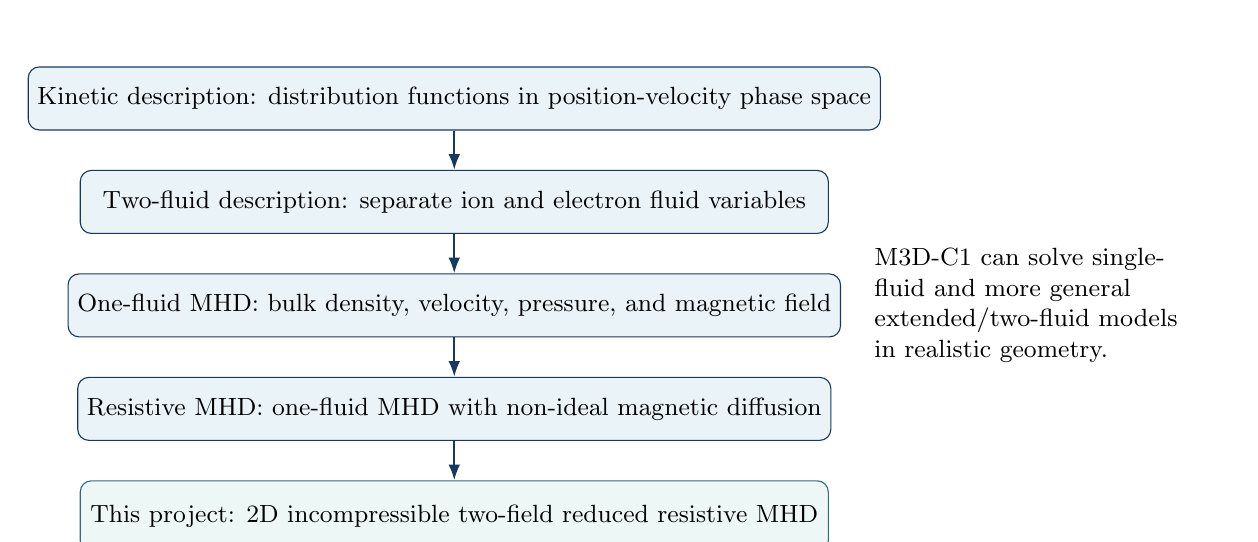
\begin{tikzpicture}[
  node distance=5mm,
  every node/.style={font=\small,align=center},
  box/.style={draw=TitleBlue,rounded corners,fill=SoftBlue,minimum width=9.5cm,minimum height=8mm},
  proj/.style={draw=AccentTeal,rounded corners,fill=SoftTeal,minimum width=9.5cm,minimum height=9mm},
  arr/.style={-{Latex[length=2mm]},thick,color=TitleBlue}
]
\node[box] (kin) {Kinetic description: distribution functions in position-velocity phase space};
\node[box,below=of kin] (two) {Two-fluid description: separate ion and electron fluid variables};
\node[box,below=of two] (one) {One-fluid MHD: bulk density, velocity, pressure, and magnetic field};
\node[box,below=of one] (res) {Resistive MHD: one-fluid MHD with non-ideal magnetic diffusion};
\node[proj,below=of res] (red) {This project: 2D incompressible two-field reduced resistive MHD};
\draw[arr] (kin)--(two);
\draw[arr] (two)--(one);
\draw[arr] (one)--(res);
\draw[arr] (res)--(red);
\node[right=3mm of one,align=left,text width=4.4cm] {M3D-C1 can solve single-fluid and more general extended/two-fluid models in realistic geometry.};
\end{tikzpicture}
\caption{A conceptual hierarchy. Each downward step discards degrees of freedom under additional assumptions. M3D-C1 is not simply the box immediately above the project model; it spans a substantially broader set of models.}
\label{fig:hierarchy}
\end{figure}

\subsection{The three claims that must remain separate}

\begin{longtable}{>{\bfseries}p{0.15\textwidth}p{0.76\textwidth}}
\toprule
Claim & Scientifically defensible meaning \\
\midrule
\endfirsthead
\toprule
Claim & Scientifically defensible meaning \\
\midrule
\endhead
A & A parameterized PINN can be tested against independently generated synthetic trajectories of a stated two-field reduced resistive-MHD model. \\
B & The inputs, outputs, metadata, diagnostics, and train/test organization can illustrate how a later workflow could accept M3D-C1 exports. \\
C & A neural surrogate accurately predicts actual M3D-C1 results over a measured domain of equilibria, closures, meshes, perturbations, and time. This claim requires genuine M3D-C1 data and lies outside the initial project. \\
\bottomrule
\end{longtable}

Module~1 provides the physical foundation for Claim~A and the vocabulary needed to describe Claim~B honestly. It provides no evidence for Claim~C.

\section{Mathematical language used throughout the module}
\label{sec:math}

This section defines the notation needed later. It is not a complete vector-calculus course; it is a compact dictionary between the mathematics and the physical statements.

\subsection{Coordinates, scalar fields, vector fields, and unit vectors}

We work first in three-dimensional Cartesian space with coordinates $(x,y,z)$. The unit vectors $\widehat{\vect{x}}$, $\widehat{\vect{y}}$, and $\widehat{\vect{z}}$ have unit length and point along the positive coordinate axes. A \emph{scalar field} assigns one number to every location and time; pressure $p(x,y,z,t)$ is an example. A \emph{vector field} assigns a vector; velocity
\begin{equation}
\vect{v}(x,y,z,t)=v_x\widehat{\vect{x}}+v_y\widehat{\vect{y}}+v_z\widehat{\vect{z}}
\end{equation}
is an example. Subscripts on a vector component, such as $v_x$, identify the component and do not denote differentiation.

The project later imposes $\partial/\partial z=0$. This means that every evolved field is independent of $z$. The $z$ direction is then called an \emph{ignorable} or \emph{out-of-plane} direction. A vector can still have a $z$ component even when its fields do not vary with $z$.

\subsection{Partial derivatives and the gradient}

The symbol
\begin{equation}
\frac{\partial f}{\partial x}\equiv f_x
\end{equation}
is the partial derivative of a scalar field $f$ with respect to $x$, holding the other independent variables fixed. We will use both forms. The gradient collects the three spatial partial derivatives into a vector:
\begin{equation}
\nabla f
=\widehat{\vect{x}}\frac{\partial f}{\partial x}
+\widehat{\vect{y}}\frac{\partial f}{\partial y}
+\widehat{\vect{z}}\frac{\partial f}{\partial z}.
\end{equation}
The gradient points in the direction of fastest local increase of $f$.

When only $x$ and $y$ derivatives are present, we write
\begin{equation}
\nabla_\perp f
=\widehat{\vect{x}}f_x+\widehat{\vect{y}}f_y.
\end{equation}
The subscript $\perp$ anticipates that this plane is perpendicular to the constant guide field introduced later.

\subsection{Divergence, curl, and Laplacian}

The divergence of a vector field measures local expansion or compression:
\begin{equation}
\nabla\cdot\vect{v}
=\frac{\partial v_x}{\partial x}
+\frac{\partial v_y}{\partial y}
+\frac{\partial v_z}{\partial z}.
\end{equation}
A flow is \emph{incompressible} when $\nabla\cdot\vect{v}=0$.

The curl measures local rotation:
\begin{equation}
\nabla\times\vect{v}
=
\begin{vmatrix}
\widehat{\vect{x}}&\widehat{\vect{y}}&\widehat{\vect{z}}\\
\partial_x&\partial_y&\partial_z\\
v_x&v_y&v_z
\end{vmatrix}.
\end{equation}
The vorticity vector is defined as $\boldsymbol{\omega}=\nabla\times\vect{v}$. In a two-dimensional in-plane flow it has only a $z$ component.

The Laplacian of a scalar is the divergence of its gradient:
\begin{equation}
\nabla^2 f\equiv\nabla\cdot\nabla f
=f_{xx}+f_{yy}+f_{zz}.
\end{equation}
In two dimensions,
\begin{equation}
\Lap f=f_{xx}+f_{yy}.
\end{equation}
Repeated subscripts denote repeated differentiation: $f_{xx}=\partial^2f/\partial x^2$.

\subsection{Local time change and material time change}

The partial derivative $\partial f/\partial t$ measures the change observed at one fixed spatial point. A moving fluid element experiences an additional change because it travels through spatial gradients. Its \emph{material derivative} is
\begin{equation}
\frac{D f}{D t}
\equiv
\frac{\partial f}{\partial t}+\vect{v}\cdot\nabla f.
\label{eq:material}
\end{equation}
The term $\vect{v}\cdot\nabla f$ is \emph{advection}: transport of $f$ by the bulk motion.

\begin{definitionbox}
Advection moves a pattern with the flow. Diffusion smooths a pattern by reducing sharp gradients. A prototype advection-diffusion equation is
\[
\frac{\partial f}{\partial t}+\vect{v}\cdot\nabla f=D\nabla^2f,
\]
where $D$ is a diffusivity with dimensions of length squared per time.
\end{definitionbox}

\subsection{Useful identities}

The derivations use the identities
\begin{align}
\nabla\cdot(\nabla\times\vect{A})&=0,\\
\nabla\times(\nabla\phi)&=0,\\
\nabla\times(\nabla\times\vect{A})
&=\nabla(\nabla\cdot\vect{A})-\nabla^2\vect{A}.
\end{align}
The first states that a field written as a curl is automatically divergence-free. The second states that a pure gradient has no curl. The third connects the curl of the current to the Laplacian of the magnetic field.

\section{From particles to a conducting fluid}
\label{sec:plasmafluid}

\subsection{What is a plasma?}

A plasma is an ionized medium containing mobile charged particles, most commonly positively charged ions and negatively charged electrons. It is not defined merely by being hot. Its defining behavior is collective: electromagnetic fields generated by many particles influence the motion of many other particles.

The \emph{Debye length} is the characteristic distance over which a plasma screens an electrostatic disturbance. On length scales much larger than this screening length, most fusion plasmas are approximately \emph{quasi-neutral}: the positive and negative charge densities nearly cancel. Quasi-neutrality does not mean that the electric field is zero. Very small departures from exact neutrality can support dynamically important electric fields.

\subsection{Three common levels of description}

\paragraph{Kinetic description.}
For each species $s$ (for example, ions or electrons), a distribution function $f_s(\vect{x},\vect{v},t)$ gives density in a six-dimensional phase space formed by three position coordinates $\vect{x}$ and three velocity coordinates $\vect{v}$. This description retains velocity-space structure, particle resonances, non-thermal populations, and many collisionless effects.

\paragraph{Fluid description.}
Velocity moments of $f_s$ produce fields in ordinary space. The zeroth moment gives number density, the first gives bulk velocity, and the second is related to pressure and temperature. A fluid model evolves a finite set of such moments and requires a \emph{closure}: an additional physical relation that approximates unevolved higher moments using the retained variables.

\paragraph{Magnetohydrodynamic description.}
MHD combines the charged species into a macroscopic conducting fluid and couples its mass, momentum, and thermodynamic evolution to reduced Maxwell equations. It is therefore a fluid theory, even though its coefficients and closures ultimately arise from particle physics.

\subsection{Two-fluid and one-fluid variables}

A two-fluid model assigns separate number densities $n_i,n_e$, velocities $\vect{v}_i,\vect{v}_e$, and pressures $p_i,p_e$ to ions and electrons. A one-fluid model forms collective variables. For a singly ionized plasma with ion mass $m_i$ much larger than electron mass $m_e$, representative definitions are
\begin{align}
\rho_{\rm d}&=m_i n_i+m_e n_e,\\
\rho_{\rm d}\vect{v}_{\rm d}&=m_i n_i\vect{v}_i+m_e n_e\vect{v}_e,\\
\vect{j}_{\rm d}&=e n_i\vect{v}_i-e n_e\vect{v}_e,
\end{align}
where $e>0$ is the elementary charge, $\rho_{\rm d}$ is mass density, $\vect{v}_{\rm d}$ is center-of-mass fluid velocity, and $\vect{j}_{\rm d}$ is electric current density. The subscript $d$ means \emph{dimensional}; these quantities carry units from the International System of Units (SI). Later, unadorned project variables will be dimensionless.

The current density measures the relative motion of positive and negative charge. The bulk velocity measures the mass-weighted common motion. They are distinct even when the plasma is approximately quasi-neutral.

\subsection{What is sacrificed in a fluid reduction?}

Fluid MHD cannot, by itself, reproduce arbitrary velocity-space distributions, wave-particle resonances, finite-orbit effects, or collisionless kinetic damping. It is useful when the desired dynamics occurs on spatial and temporal scales sufficiently large compared with microscopic kinetic scales, and when a suitable closure represents the discarded moments. ``MHD is valid'' is never an absolute statement; it is a statement about the phenomena and scale range under study \cite{Goedbloed2004}.

\begin{checkpointbox}
The distribution function is a field on phase space. The MHD variables are also fields, but they live on ordinary space and time. MHD does not stop being a field theory when it stops explicitly evolving the distribution function.
\end{checkpointbox}

\section{Physical building blocks: electromagnetism and fluid conservation}
\label{sec:buildingblocks}

\subsection{Lorentz force}

A particle of charge $q$ and velocity $\vect{u}$ experiences the Lorentz force
\begin{equation}
\vect{F}=q\left(\vect{E}_{\rm d}+\vect{u}\times\vect{B}_{\rm d}\right),
\end{equation}
where $\vect{E}_{\rm d}$ is the electric field and $\vect{B}_{\rm d}$ is the magnetic field. In a fluid, the corresponding macroscopic electromagnetic force density is
\begin{equation}
\vect{f}_{\rm EM}=\rho_{q,\rm d}\vect{E}_{\rm d}+\vect{j}_{\rm d}\times\vect{B}_{\rm d},
\end{equation}
where $\rho_{q,\rm d}$ is charge density. In nonrelativistic quasi-neutral MHD, the electric-force-density term is smaller in the standard ordering and the dominant macroscopic force is $\vect{j}_{\rm d}\times\vect{B}_{\rm d}$.

\subsection{Reduced Maxwell equations used by MHD}

The MHD model uses
\begin{align}
\frac{\partial\vect{B}_{\rm d}}{\partial t_{\rm d}}
&=-\nabla_{\rm d}\times\vect{E}_{\rm d}
&&\text{(Faraday's law)},\label{eq:faraday}\\
\nabla_{\rm d}\times\vect{B}_{\rm d}
&=\mu_0\vect{j}_{\rm d}
&&\text{(Ampere's law without displacement current)},\label{eq:ampere}\\
\nabla_{\rm d}\cdot\vect{B}_{\rm d}&=0
&&\text{(absence of magnetic monopoles)}.\label{eq:divB}
\end{align}
Here $\mu_0$ is the permeability of free space. The displacement current is neglected because standard MHD describes nonrelativistic motions with characteristic speeds much smaller than the speed of light \cite{Goedbloed2004}.

\subsection{Conservation of mass}

For mass density $\rho_{\rm d}$ and fluid velocity $\vect{v}_{\rm d}$,
\begin{equation}
\frac{\partial\rho_{\rm d}}{\partial t_{\rm d}}
+\nabla_{\rm d}\cdot(\rho_{\rm d}\vect{v}_{\rm d})=0.
\label{eq:continuity_dim}
\end{equation}
Using the material derivative,
\begin{equation}
\frac{D\rho_{\rm d}}{Dt_{\rm d}}+\rho_{\rm d}\nabla_{\rm d}\cdot\vect{v}_{\rm d}=0.
\end{equation}
Thus density of a moving fluid element remains constant if the flow is incompressible.

\subsection{Conservation of momentum}

A simple viscous one-fluid momentum equation is
\begin{equation}
\rho_{\rm d}\left(
\frac{\partial\vect{v}_{\rm d}}{\partial t_{\rm d}}
+\vect{v}_{\rm d}\cdot\nabla_{\rm d}\vect{v}_{\rm d}
\right)
=-\nabla_{\rm d}p_{\rm d}
+\vect{j}_{\rm d}\times\vect{B}_{\rm d}
+\rho_{\rm d}\nu_{\rm d}\nabla_{\rm d}^{2}\vect{v}_{\rm d}.
\label{eq:momentum_dim}
\end{equation}
The scalar $p_{\rm d}$ is isotropic pressure and $\nu_{\rm d}$ is kinematic viscosity, with units $\unit{m^2\,s^{-1}}$. The left-hand side is mass density times acceleration. On the right are the pressure-gradient force, Lorentz force, and a simplified viscous force.

Production extended-MHD models may use an anisotropic viscous stress tensor rather than the scalar Laplacian term in Eq.~\eqref{eq:momentum_dim}. The scalar form is a deliberate project assumption.

\subsection{Thermodynamic closure}

The fields $\rho_{\rm d}$, $\vect{v}_{\rm d}$, $p_{\rm d}$, and $\vect{B}_{\rm d}$ do not form a closed compressible system without an equation for pressure or internal energy. For example, an adiabatic ideal-gas closure has
\begin{equation}
\frac{D p_{\rm d}}{Dt_{\rm d}}+\gamma p_{\rm d}\nabla_{\rm d}\cdot\vect{v}_{\rm d}=0,
\end{equation}
where $\gamma$ is the ratio of specific heats. Resistive and viscous heating and thermal conduction add further terms.

The project removes this equation by imposing constant density and incompressibility and then taking the curl of the momentum equation. Pressure remains physically present as the field that enforces incompressibility, but it disappears from the vorticity evolution because the curl of a gradient is zero.

\section{One-fluid resistive magnetohydrodynamics}
\label{sec:fullmhd}

\subsection{Ohm's law in a moving conducting fluid}

The simplest resistive Ohm's law is
\begin{equation}
\vect{E}_{\rm d}+\vect{v}_{\rm d}\times\vect{B}_{\rm d}
=\rho_{\Omega}\vect{j}_{\rm d}.
\label{eq:ohm_dim}
\end{equation}
The symbol $\rho_{\Omega}$ denotes \emph{electrical resistivity}, with International System of Units (SI) units $\unit{\Omega\,m}$. It is the inverse of electrical conductivity. The combination $\vect{E}_{\rm d}+\vect{v}_{\rm d}\times\vect{B}_{\rm d}$ is the electric field measured in the moving-fluid frame in the nonrelativistic limit.

If $\rho_{\Omega}=0$, Eq.~\eqref{eq:ohm_dim} becomes the ideal-MHD condition
\begin{equation}
\vect{E}_{\rm d}+\vect{v}_{\rm d}\times\vect{B}_{\rm d}=0.
\label{eq:idealohm}
\end{equation}

\begin{warningbox}
Electrical resistivity $\rho_{\Omega}$, dimensional magnetic diffusivity $\eta_{\rm m}$, and dimensionless project diffusivity $\eta$ are three related but different quantities:
\[
\eta_{\rm m}=\frac{\rho_{\Omega}}{\mu_0},
\qquad
\eta=\frac{\eta_{\rm m}}{L_0V_A}.
\]
The project symbol $\eta$ never carries units of $\unit{\Omega\,m}$.
\end{warningbox}

\subsection{Derivation of the resistive induction equation}

Insert Ohm's law into Faraday's law:
\begin{align}
\frac{\partial\vect{B}_{\rm d}}{\partial t_{\rm d}}
&=-\nabla_{\rm d}\times\vect{E}_{\rm d}\\
&=\nabla_{\rm d}\times(\vect{v}_{\rm d}\times\vect{B}_{\rm d})
-\nabla_{\rm d}\times(\rho_{\Omega}\vect{j}_{\rm d}).
\end{align}
For constant $\rho_{\Omega}$, Ampere's law gives
\begin{align}
-\nabla_{\rm d}\times(\rho_{\Omega}\vect{j}_{\rm d})
&=-\frac{\rho_{\Omega}}{\mu_0}
\nabla_{\rm d}\times(\nabla_{\rm d}\times\vect{B}_{\rm d})\\
&=\frac{\rho_{\Omega}}{\mu_0}\nabla_{\rm d}^{2}\vect{B}_{\rm d},
\end{align}
where $\nabla\cdot\vect{B}=0$ was used. Defining magnetic diffusivity
\begin{equation}
\eta_{\rm m}\equiv\frac{\rho_{\Omega}}{\mu_0},
\end{equation}
we obtain
\begin{equation}
\frac{\partial\vect{B}_{\rm d}}{\partial t_{\rm d}}
=\nabla_{\rm d}\times(\vect{v}_{\rm d}\times\vect{B}_{\rm d})
+\eta_{\rm m}\nabla_{\rm d}^{2}\vect{B}_{\rm d}.
\label{eq:induction_dim}
\end{equation}

The first term transports and deforms magnetic field with the fluid. The second term diffuses magnetic field and permits magnetic topology to change. In an almost ideal plasma, $\eta_{\rm m}$ can be small while $\eta_{\rm m}\nabla^2\vect{B}$ remains important inside a thin current sheet, where spatial derivatives become large \cite{Goedbloed2004,Goedbloed2010}.

\subsection{The one-fluid resistive-MHD set}

In its simplified form, the parent model contains
\begin{align}
\frac{\partial\rho_{\rm d}}{\partial t_{\rm d}}
+\nabla_{\rm d}\cdot(\rho_{\rm d}\vect{v}_{\rm d})&=0,\\
\rho_{\rm d}\frac{D\vect{v}_{\rm d}}{Dt_{\rm d}}
&=-\nabla_{\rm d}p_{\rm d}+\vect{j}_{\rm d}\times\vect{B}_{\rm d}
+\rho_{\rm d}\nu_{\rm d}\nabla_{\rm d}^2\vect{v}_{\rm d},\\
\frac{\partial\vect{B}_{\rm d}}{\partial t_{\rm d}}
&=\nabla_{\rm d}\times(\vect{v}_{\rm d}\times\vect{B}_{\rm d})
+\eta_{\rm m}\nabla_{\rm d}^2\vect{B}_{\rm d},\\
\nabla_{\rm d}\cdot\vect{B}_{\rm d}&=0,\\
\mu_0\vect{j}_{\rm d}&=\nabla_{\rm d}\times\vect{B}_{\rm d},
\end{align}
plus a thermodynamic closure. This is the physical parent from which the project model is reduced.

\subsection{Ideal versus resistive MHD}

Ideal MHD sets electrical resistivity and viscosity to zero. It is not the entirety of plasma physics. It is a particular nondissipative fluid limit. Resistive MHD retains finite electrical resistivity, producing Ohmic heating and magnetic diffusion. Viscous-resistive MHD also retains viscous diffusion of momentum or vorticity.

The word \emph{non-ideal} is broader than \emph{resistive}. Hall drift, electron-pressure terms, electron inertia, anisotropic stresses, and kinetic effects can all violate the ideal Ohm's law. The present project retains only scalar resistive and viscous departures from the ideal two-field dynamics.

\section{Assumptions that define the project reduction}
\label{sec:reduction}

The final equations are not guessed. They follow from the parent model after the assumptions below are imposed. Each assumption has both a mathematical consequence and a physical cost.

\begin{longtable}{p{0.23\textwidth}p{0.32\textwidth}p{0.35\textwidth}}
\toprule
Assumption & Mathematical consequence & Physics omitted or restricted \\
\midrule
\endfirsthead
\toprule
Assumption & Mathematical consequence & Physics omitted or restricted \\
\midrule
\endhead
Two-dimensional Cartesian domain & $\partial_z=0$; evolved fields depend on $(x,y,t)$ only & Toroidal geometry, three-dimensional variation, and parallel structure \\
Constant mass density $\rho_0$ & Density equation becomes redundant & Compression, density waves, stratification, and density transport \\
Incompressible flow & $\nabla_\perp\cdot\vect{v}_\perp=0$ & Fast and slow magnetosonic compression and acoustic dynamics \\
Strong, uniform guide field & $\vect{B}=B_g\widehat{\vect{z}}+\vect{B}_\perp$ & Evolution of guide-field magnitude and associated compressional physics \\
Perpendicular in-plane flow & $v_z=0$ & Parallel flow and parallel momentum dynamics \\
Scalar constant resistivity & One coefficient $\eta_{\rm m}$ multiplies $\nabla^2\vect{B}$ & Temperature-dependent, anisotropic, anomalous, and tensor resistivity \\
Scalar constant viscosity & One coefficient $\nu_{\rm d}$ multiplies $\nabla^2\vect{v}$ & Anisotropic collisional stress, finite-gyroradius viscous corrections, and spatially varying transport \\
No separate pressure/energy evolution & Curl of momentum removes $p$ & Temperature, heat conduction, Ohmic heating feedback, and pressure-driven modes \\
Doubly periodic boundaries & No physical wall or boundary flux & Wall currents, vacuum region, separatrix, material interfaces, and sheath physics \\
\bottomrule
\end{longtable}

\subsection{Two-dimensional geometry and the guide field}

Let the magnetic field be
\begin{equation}
\vect{B}_{\rm d}=B_g\widehat{\vect{z}}+\vect{B}_{\perp,\rm d},
\end{equation}
where $B_g$ is a constant guide field and $\vect{B}_{\perp,\rm d}$ lies in the $x$-$y$ plane. All fields satisfy $\partial_z=0$. Because the guide field is spatially uniform, it produces no current. Because the current in this strict two-dimensional model points in the $z$ direction, its cross product with $B_g\widehat{\vect{z}}$ vanishes. The guide field motivates the reduced ordering but does not explicitly appear in the final two-dimensional equations.

\begin{warningbox}
The full three-dimensional two-field reduced-MHD equations normally contain derivatives along the guide field. Setting $\partial_z=0$ removes those terms. The project system is therefore the strictly two-dimensional limit of two-field reduced MHD and is also mathematically equivalent, up to sign and normalization conventions, to two-dimensional incompressible resistive MHD with a uniform guide field.
\end{warningbox}

\subsection{Constant density and incompressibility}

Set $\rho_{\rm d}=\rho_0$, a positive constant. The continuity equation becomes
\begin{equation}
\rho_0\nabla_{\rm d}\cdot\vect{v}_{\rm d}=0,
\end{equation}
so
\begin{equation}
\nabla_{\rm d}\cdot\vect{v}_{\rm d}=0.
\end{equation}
Incompressibility does not mean that the velocity is spatially uniform. It means that the local volume of a moving fluid element does not change. The flow may still shear, stretch, rotate, and form small scales.

\subsection{Why pressure disappears but is not physically absent}

Pressure in incompressible flow adjusts so that the velocity remains divergence-free. If one solves directly for velocity, pressure is a Lagrange-multiplier-like field coupled through an elliptic equation. The project instead takes the curl of momentum. Since
\begin{equation}
\nabla\times(-\nabla p)=0,
\end{equation}
pressure disappears from the vorticity equation. This is a mathematical elimination of the pressure gradient, not an assertion that the plasma has zero pressure.

\section{Flux and stream functions: building divergence-free fields}
\label{sec:potentials}

\subsection{Magnetic-flux function}

Define a dimensional scalar magnetic-flux function $\psi_{\rm d}(x_{\rm d},y_{\rm d},t_{\rm d})$ by
\begin{equation}
\vect{B}_{\perp,\rm d}
=\nabla_{\rm d}\psi_{\rm d}\times\widehat{\vect{z}}.
\label{eq:Bpsi_dim}
\end{equation}
The cross product gives
\begin{equation}
\vect{B}_{\perp,\rm d}
=\left(\frac{\partial\psi_{\rm d}}{\partial y_{\rm d}},
-\frac{\partial\psi_{\rm d}}{\partial x_{\rm d}},0\right).
\label{eq:Bcomponents_dim}
\end{equation}
Because $\vect{B}_{\perp,\rm d}=\nabla\times(\psi_{\rm d}\widehat{\vect{z}})$, it is divergence-free automatically:
\begin{equation}
\nabla_{\rm d}\cdot\vect{B}_{\perp,\rm d}=0.
\end{equation}
The SI unit of $\psi_{\rm d}$ is tesla-meter, $\unit{T\,m}$, which is magnetic flux per unit distance in the ignorable $z$ direction.

The magnetic field is tangent to contours of $\psi_{\rm d}$ because
\begin{equation}
\vect{B}_{\perp,\rm d}\cdot\nabla_{\rm d}\psi_{\rm d}=0.
\end{equation}
Thus, in a two-dimensional plot, contour lines of $\psi$ are magnetic-field lines in the plane.

\subsection{Flow stream function}

Define a dimensional stream function $U_{\rm d}$ by
\begin{equation}
\vect{v}_{\perp,\rm d}
=\widehat{\vect{z}}\times\nabla_{\rm d}U_{\rm d}.
\label{eq:vU_dim}
\end{equation}
Therefore,
\begin{equation}
\vect{v}_{\perp,\rm d}
=\left(-\frac{\partial U_{\rm d}}{\partial y_{\rm d}},
\frac{\partial U_{\rm d}}{\partial x_{\rm d}},0\right).
\label{eq:vcomponents_dim}
\end{equation}
This field is also divergence-free identically. The SI unit of $U_{\rm d}$ is $\unit{m^2\,s^{-1}}$, because one spatial derivative of $U_{\rm d}$ must have velocity units.

\begin{conventionbox}
After nondimensionalization, the project uses
\[
\boxed{
\vect{B}_{\perp}=\nabla\psi\times\widehat{\vect{z}}
=(\psi_y,-\psi_x),
\qquad
\vect{v}_{\perp}=\widehat{\vect{z}}\times\nabla U
=(-U_y,U_x).}
\]
Changing either cross-product order changes signs throughout the model. These definitions are frozen.
\end{conventionbox}

\subsection{Current density from the flux function}

Ampere's law gives an out-of-plane current density. From Eq.~\eqref{eq:Bcomponents_dim},
\begin{align}
\mu_0 j_{z,\rm d}
&=(\nabla_{\rm d}\times\vect{B}_{\perp,\rm d})_z\\
&=\frac{\partial B_{y,\rm d}}{\partial x_{\rm d}}
-\frac{\partial B_{x,\rm d}}{\partial y_{\rm d}}\\
&=-\frac{\partial^2\psi_{\rm d}}{\partial x_{\rm d}^2}
-\frac{\partial^2\psi_{\rm d}}{\partial y_{\rm d}^2}\\
&=-\nabla_{\perp,\rm d}^{2}\psi_{\rm d}.
\label{eq:jpsi_dim}
\end{align}
The dimensionless project current variable will be scaled so that
\begin{equation}
\boxed{J=-\Lap\psi.}
\label{eq:Jdef}
\end{equation}
The scalar $J$ is proportional to physical current density $j_{z,\rm d}$; it is not itself an SI current density.

\subsection{Vorticity from the stream function}

The out-of-plane vorticity is
\begin{align}
\omega_{z,\rm d}
&=(\nabla_{\rm d}\times\vect{v}_{\perp,\rm d})_z\\
&=\frac{\partial v_{y,\rm d}}{\partial x_{\rm d}}
-\frac{\partial v_{x,\rm d}}{\partial y_{\rm d}}\\
&=\frac{\partial^2 U_{\rm d}}{\partial x_{\rm d}^2}
+\frac{\partial^2 U_{\rm d}}{\partial y_{\rm d}^2}\\
&=\nabla_{\perp,\rm d}^{2}U_{\rm d}.
\end{align}
After nondimensionalization,
\begin{equation}
\boxed{\omega=\Lap U.}
\label{eq:omegadef}
\end{equation}

\begin{checkpointbox}
The signs are not arbitrary once the vector definitions are fixed. The chain is
\[
\vect{B}_\perp=(\psi_y,-\psi_x)
\Rightarrow J=-\nabla^2\psi,
\qquad
\vect{v}_\perp=(-U_y,U_x)
\Rightarrow\omega=+\nabla^2U.
\]
The opposite signs of $J$ and $\omega$ arise from the opposite cross-product order in the definitions of $\vect{B}_\perp$ and $\vect{v}_\perp$.
\end{checkpointbox}


\section{The Poisson bracket and two-dimensional advection}
\label{sec:bracket}

\subsection{Definition}

For two scalar fields $f(x,y)$ and $g(x,y)$, define the Poisson bracket
\begin{equation}
\boxed{
\bracket{f}{g}
\equiv f_x g_y-f_y g_x.}
\label{eq:bracketdef}
\end{equation}
The name ``Poisson bracket'' is shared with Hamiltonian mechanics. Here it is a compact notation for a particular combination of two-dimensional derivatives.

\subsection{The bracket is advection by the stream-function flow}

Using $\vect{v}_\perp=(-U_y,U_x)$,
\begin{align}
\vect{v}_\perp\cdot\nabla f
&=(-U_y)f_x+(U_x)f_y\\
&=U_xf_y-U_yf_x\\
&=\bracket{U}{f}.
\label{eq:vadvectionbracket}
\end{align}
Therefore
\begin{equation}
\frac{Df}{Dt}=f_t+\bracket{U}{f}.
\end{equation}
The nonlinear terms $[U,\psi]$ and $[U,\omega]$ in the final equations are simply advection of magnetic flux and vorticity by the incompressible flow.

Similarly, using $\vect{B}_\perp=(\psi_y,-\psi_x)$,
\begin{align}
\vect{B}_\perp\cdot\nabla f
&=\psi_yf_x-\psi_xf_y\\
&=\bracket{f}{\psi}
=-\bracket{\psi}{f}.
\label{eq:Badvectionbracket}
\end{align}

\subsection{Algebraic properties}

The bracket satisfies:
\begin{align}
\bracket{f}{g}&=-\bracket{g}{f}
&&\text{(antisymmetry)},\label{eq:bracketantisym}\\
\bracket{f}{f}&=0,\\
\bracket{f}{gh}&=g\bracket{f}{h}+h\bracket{f}{g}
&&\text{(product rule)},\\
\bracket{f}{\bracket{g}{h}}
+\bracket{g}{\bracket{h}{f}}
+\bracket{h}{\bracket{f}{g}}&=0
&&\text{(Jacobi identity)}.
\end{align}
The Jacobi identity is structurally important in Hamiltonian formulations, although the first implementation does not need to evaluate it explicitly.

\subsection{Integral identities on a periodic domain}

Let $\Omega=[0,L_x)\times[0,L_y)$, with all fields periodic in both directions. Integration by parts produces no boundary contribution. Consequently,
\begin{align}
\int_\Omega \bracket{f}{g}\,\dd A&=0,\label{eq:intbracketzero}\\
\int_\Omega f\bracket{g}{h}\,\dd A
&=\int_\Omega g\bracket{h}{f}\,\dd A
=\int_\Omega h\bracket{f}{g}\,\dd A.
\label{eq:bracketcyclic}
\end{align}
Equation~\eqref{eq:bracketcyclic} is the cyclic bracket identity. It is central to the energy proof in Section~\ref{sec:energy}.

To see why Eq.~\eqref{eq:intbracketzero} holds, write
\begin{equation}
\bracket{f}{g}
=\frac{\partial}{\partial x}(f g_y)
-\frac{\partial}{\partial y}(f g_x).
\end{equation}
The integral of each total derivative across one periodic direction vanishes because the values at the two identified faces are equal.

\section{Derivation of the magnetic-flux equation}
\label{sec:fluxderivation}

The first project equation is
\begin{equation}
\psi_t+\bracket{U}{\psi}=\eta\Lap\psi.
\label{eq:fluxproject_preview}
\end{equation}
We derive it first in dimensional form, then nondimensionalize it in Section~\ref{sec:nondim}.

\subsection{Vector-potential gauge used in two dimensions}

Because
\begin{equation}
\vect{B}_{\perp,\rm d}=\nabla_{\rm d}\times
(\psi_{\rm d}\widehat{\vect{z}}),
\end{equation}
we may use a vector potential $\vect{A}_{\rm d}=\psi_{\rm d}\widehat{\vect{z}}$. The electric field can be written
\begin{equation}
\vect{E}_{\rm d}
=-\frac{\partial\vect{A}_{\rm d}}{\partial t_{\rm d}}
-\nabla_{\rm d}\Phi_{\rm d},
\end{equation}
where $\Phi_{\rm d}$ is electrostatic potential. Since $\partial_z\Phi_{\rm d}=0$, the out-of-plane component is
\begin{equation}
E_{z,\rm d}=-\frac{\partial\psi_{\rm d}}{\partial t_{\rm d}}.
\label{eq:Ezpsit}
\end{equation}

\subsection{The out-of-plane component of Ohm's law}

The $z$ component of $\vect{v}\times\vect{B}$ is
\begin{align}
(\vect{v}_{\perp,\rm d}\times\vect{B}_{\perp,\rm d})_z
&=v_{x,\rm d}B_{y,\rm d}-v_{y,\rm d}B_{x,\rm d}\\
&=(-U_{{\rm d},y})(-\psi_{{\rm d},x})
-(U_{{\rm d},x})(\psi_{{\rm d},y})\\
&=-\bracket{U_{\rm d}}{\psi_{\rm d}}_{\rm d}.
\end{align}
The subscript on the bracket indicates derivatives with respect to dimensional coordinates. The $z$ component of resistive Ohm's law is therefore
\begin{equation}
-\psi_{{\rm d},t}
-\bracket{U_{\rm d}}{\psi_{\rm d}}_{\rm d}
=\rho_\Omega j_{z,\rm d}.
\end{equation}
Using $\mu_0j_{z,\rm d}=-\nabla_{\perp,\rm d}^2\psi_{\rm d}$ and $\eta_{\rm m}=\rho_\Omega/\mu_0$ gives
\begin{equation}
\boxed{
\frac{\partial\psi_{\rm d}}{\partial t_{\rm d}}
+\bracket{U_{\rm d}}{\psi_{\rm d}}_{\rm d}
=\eta_{\rm m}\nabla_{\perp,\rm d}^{2}\psi_{\rm d}.}
\label{eq:flux_dim}
\end{equation}

\subsection{Physical interpretation}

The left-hand side is the material derivative of $\psi_{\rm d}$:
\begin{equation}
\frac{D\psi_{\rm d}}{Dt_{\rm d}}
=\frac{\partial\psi_{\rm d}}{\partial t_{\rm d}}
+\vect{v}_{\perp,\rm d}\cdot\nabla_{\rm d}\psi_{\rm d}.
\end{equation}
Thus
\begin{equation}
\frac{D\psi_{\rm d}}{Dt_{\rm d}}
=\eta_{\rm m}\nabla_{\perp,\rm d}^{2}\psi_{\rm d}.
\end{equation}
In the ideal limit $\eta_{\rm m}=0$, each moving fluid element retains its value of $\psi_{\rm d}$. This is the two-dimensional expression of frozen-in magnetic flux. At finite resistivity, diffusion changes the flux carried by a fluid element.

Using $J=-\nabla^2\psi$, the dimensionless resistive source is
\begin{equation}
\eta\nabla^2\psi=-\eta J.
\end{equation}
Therefore resistive evolution is strongest where the magnitude of the current variable is large.

\section{Derivation of the vorticity equation}
\label{sec:vorticityderivation}

The second project equation is
\begin{equation}
\omega_t+\bracket{U}{\omega}
=\bracket{J}{\psi}+\nu\Lap\omega.
\label{eq:vorticityproject_preview}
\end{equation}
It is the out-of-plane curl of the momentum equation.

\subsection{Begin with incompressible momentum balance}

With constant density $\rho_0$,
\begin{equation}
\frac{\partial\vect{v}_{\rm d}}{\partial t_{\rm d}}
+\vect{v}_{\rm d}\cdot\nabla_{\rm d}\vect{v}_{\rm d}
=-\frac{1}{\rho_0}\nabla_{\rm d}p_{\rm d}
+\frac{1}{\rho_0}\vect{j}_{\rm d}\times\vect{B}_{\rm d}
+\nu_{\rm d}\nabla_{\rm d}^{2}\vect{v}_{\rm d}.
\label{eq:momentum_incompressible}
\end{equation}
Take $\nabla_{\rm d}\times$ of every term and select the $z$ component.

\subsection{Time derivative}

Curl and the time derivative commute for smooth fields:
\begin{equation}
\left[\nabla_{\rm d}\times
\frac{\partial\vect{v}_{\rm d}}{\partial t_{\rm d}}\right]_z
=\frac{\partial\omega_{z,\rm d}}{\partial t_{\rm d}}.
\end{equation}

\subsection{Nonlinear inertia becomes vorticity advection}

For incompressible two-dimensional flow,
\begin{equation}
\left[\nabla_{\rm d}\times
(\vect{v}_{\rm d}\cdot\nabla_{\rm d}\vect{v}_{\rm d})\right]_z
=\vect{v}_{\rm d}\cdot\nabla_{\rm d}\omega_{z,\rm d}.
\end{equation}
Using the stream function,
\begin{equation}
\vect{v}_{\rm d}\cdot\nabla_{\rm d}\omega_{z,\rm d}
=\bracket{U_{\rm d}}{\omega_{z,\rm d}}_{\rm d}.
\end{equation}

One route to the identity is the vector decomposition
\begin{equation}
(\vect{v}\cdot\nabla)\vect{v}
=\nabla\left(\frac{|\vect{v}|^2}{2}\right)
-\vect{v}\times\boldsymbol{\omega}.
\end{equation}
The first term has zero curl; the second produces vorticity transport in the two-dimensional incompressible limit.

\subsection{Pressure vanishes under curl}

Because $\rho_0$ is constant,
\begin{equation}
\nabla_{\rm d}\times\left(-\frac{1}{\rho_0}\nabla_{\rm d}p_{\rm d}\right)=0.
\end{equation}
If density were spatially variable, the curl of $-(1/\rho)\nabla p$ would generally not vanish. It would contain \emph{baroclinic vorticity generation}, which occurs when pressure and density gradients are not parallel. Constant density is therefore essential to this simple reduction.

\subsection{Lorentz force becomes the magnetic bracket}

The current is $\vect{j}_{\rm d}=j_{z,\rm d}\widehat{\vect{z}}$ and the in-plane magnetic field is $\vect{B}_{\perp,\rm d}=(\psi_y,-\psi_x,0)$. Hence
\begin{align}
\vect{j}_{\rm d}\times\vect{B}_{\perp,\rm d}
&=j_{z,\rm d}\widehat{\vect{z}}
\times(\psi_y\widehat{\vect{x}}-\psi_x\widehat{\vect{y}})\\
&=j_{z,\rm d}\nabla_{\rm d}\psi_{\rm d}.
\label{eq:lorentzgradpsi}
\end{align}
Its out-of-plane curl is
\begin{align}
\left[\nabla_{\rm d}\times
(j_{z,\rm d}\nabla_{\rm d}\psi_{\rm d})\right]_z
&=\frac{\partial j_{z,\rm d}}{\partial x_{\rm d}}
\frac{\partial\psi_{\rm d}}{\partial y_{\rm d}}
-\frac{\partial j_{z,\rm d}}{\partial y_{\rm d}}
\frac{\partial\psi_{\rm d}}{\partial x_{\rm d}}\\
&=\bracket{j_{z,\rm d}}{\psi_{\rm d}}_{\rm d}.
\end{align}
The Lorentz force therefore generates vorticity through spatial misalignment of current-density and flux contours. If $j_{z,\rm d}$ is a function of $\psi_{\rm d}$ alone, then their gradients are parallel and the bracket vanishes.

\subsection{Viscosity diffuses vorticity}

For constant $\nu_{\rm d}$,
\begin{equation}
\left[\nabla_{\rm d}\times
(\nu_{\rm d}\nabla_{\rm d}^{2}\vect{v}_{\rm d})\right]_z
=\nu_{\rm d}\nabla_{\perp,\rm d}^{2}\omega_{z,\rm d}.
\end{equation}

\subsection{Dimensional vorticity equation}

Combining the terms gives
\begin{equation}
\boxed{
\frac{\partial\omega_{z,\rm d}}{\partial t_{\rm d}}
+\bracket{U_{\rm d}}{\omega_{z,\rm d}}_{\rm d}
=\frac{1}{\rho_0}\bracket{j_{z,\rm d}}{\psi_{\rm d}}_{\rm d}
+\nu_{\rm d}\nabla_{\perp,\rm d}^{2}\omega_{z,\rm d}.}
\label{eq:vorticity_dim}
\end{equation}
Alfv\'en normalization will turn the coefficient of the magnetic bracket into unity.

\begin{checkpointbox}
The two nonlinear brackets have different jobs:
\begin{itemize}
  \item $[U,\omega]$ transports existing vorticity with the fluid;
  \item $[J,\psi]$ is the curl of the Lorentz force and can generate or redistribute vorticity.
\end{itemize}
Neither bracket is a dissipative term. Their domain integrals vanish under periodic boundary conditions.
\end{checkpointbox}

\section{Nondimensionalization and characteristic time scales}
\label{sec:nondim}

\subsection{Why nondimensionalize?}

Nondimensionalization replaces quantities carrying SI units with ratios to chosen reference scales. It has four benefits here:
\begin{enumerate}[label=(\alph*)]
  \item it exposes the relative strength of physical mechanisms;
  \item it reduces the number of independent coefficients;
  \item it makes parameter ranges portable between physical systems with similar dimensionless numbers; and
  \item it places neural-network inputs and outputs on more manageable physical scales.
\end{enumerate}
Nondimensionalization is a physical rescaling. It is not the same as later machine-learning standardization or min-max scaling.

\subsection{Reference scales}

Choose positive dimensional scales:
\begin{itemize}
  \item $L_0$: characteristic perpendicular length;
  \item $B_0$: characteristic in-plane magnetic-field magnitude;
  \item $\rho_0$: constant mass density;
  \item $V_A$: Alfv\'en speed; and
  \item $t_A$: Alfv\'en time.
\end{itemize}
The Alfv\'en speed is
\begin{equation}
V_A\equiv\frac{B_0}{\sqrt{\mu_0\rho_0}},
\label{eq:alfvenspeed}
\end{equation}
and the Alfv\'en time is
\begin{equation}
t_A\equiv\frac{L_0}{V_A}.
\label{eq:alfventime}
\end{equation}
It is the time for a disturbance traveling at $V_A$ to traverse the reference length $L_0$.

\subsection{Dimensionless variables}

Define
\begin{align}
x_{\rm d}&=L_0x,&y_{\rm d}&=L_0y,&t_{\rm d}&=t_At,\\
\psi_{\rm d}&=B_0L_0\psi,&
U_{\rm d}&=V_AL_0U,\\
\vect{B}_{\perp,\rm d}&=B_0\vect{B}_\perp,&
\vect{v}_{\perp,\rm d}&=V_A\vect{v}_\perp,\\
j_{z,\rm d}&=\frac{B_0}{\mu_0L_0}J,&
\omega_{z,\rm d}&=\frac{V_A}{L_0}\omega.
\end{align}
Spatial and temporal derivatives transform as
\begin{equation}
\nabla_{\rm d}=\frac{1}{L_0}\nabla,
\qquad
\frac{\partial}{\partial t_{\rm d}}
=\frac{1}{t_A}\frac{\partial}{\partial t}.
\end{equation}

Substitution into Eq.~\eqref{eq:jpsi_dim} gives
\begin{equation}
J=-\Lap\psi,
\end{equation}
and substitution into the vorticity definition gives
\begin{equation}
\omega=\Lap U.
\end{equation}

\subsection{Dimensionless diffusivities}

The flux equation becomes
\begin{equation}
\psi_t+\bracket{U}{\psi}
=\underbrace{\frac{\eta_{\rm m}}{L_0V_A}}_{\displaystyle\eta}\Lap\psi.
\end{equation}
Thus
\begin{equation}
\boxed{\eta\equiv\frac{\eta_{\rm m}}{L_0V_A}.}
\label{eq:eta_nondim}
\end{equation}

For the magnetic term in the vorticity equation, use $B_0^2/(\mu_0\rho_0)=V_A^2$. The coefficient becomes exactly one. The viscous coefficient is
\begin{equation}
\boxed{\nu\equiv\frac{\nu_{\rm d}}{L_0V_A}.}
\label{eq:nu_nondim}
\end{equation}

\subsection{Lundquist, Reynolds, and magnetic Prandtl numbers}

The Alfv\'enic Lundquist number is
\begin{equation}
S\equiv\frac{L_0V_A}{\eta_{\rm m}}=\frac{1}{\eta}.
\label{eq:lundquist}
\end{equation}
The fluid Reynolds number based on $V_A$ is
\begin{equation}
\mathrm{Re}\equiv\frac{L_0V_A}{\nu_{\rm d}}=\frac{1}{\nu}.
\label{eq:reynolds}
\end{equation}
The magnetic Prandtl number is
\begin{equation}
\mathrm{Pm}\equiv\frac{\nu_{\rm d}}{\eta_{\rm m}}
=\frac{\nu}{\eta}=\frac{S}{\mathrm{Re}}.
\label{eq:pm}
\end{equation}

A magnetic Reynolds number based on an actual characteristic flow speed $V_0$ is
\begin{equation}
\mathrm{Rm}\equiv\frac{L_0V_0}{\eta_{\rm m}}.
\end{equation}
It equals $S$ only when $V_0=V_A$. The project uses Alfv\'en normalization, so $1/\eta$ is most precisely called the Lundquist number, although literature sometimes loosely refers to it as a magnetic Reynolds number.

\subsection{Time-scale interpretation}

The dimensional diffusion times are
\begin{align}
t_\eta&=\frac{L_0^2}{\eta_{\rm m}},\\
t_\nu&=\frac{L_0^2}{\nu_{\rm d}}.
\end{align}
Relative to $t_A$,
\begin{equation}
\frac{t_\eta}{t_A}=S=\frac{1}{\eta},
\qquad
\frac{t_\nu}{t_A}=\mathrm{Re}=\frac{1}{\nu}.
\end{equation}

\begin{longtable}{p{0.22\textwidth}p{0.25\textwidth}p{0.42\textwidth}}
\toprule
Scale & Expression & Meaning \\
\midrule
\endfirsthead
\toprule
Scale & Expression & Meaning \\
\midrule
\endhead
Alfv\'en time & $t_A=L_0/V_A$ & Ideal magnetic-tension response across $L_0$ \\
Resistive time & $t_\eta=L_0^2/\eta_{\rm m}$ & Diffusive smoothing of magnetic structure on scale $L_0$ \\
Viscous time & $t_\nu=L_0^2/\nu_{\rm d}$ & Diffusive smoothing of velocity on scale $L_0$ \\
Lundquist number & $S=t_\eta/t_A$ & Separation between resistive and Alfv\'enic times \\
Reynolds number & $\mathrm{Re}=t_\nu/t_A$ & Separation between viscous and Alfv\'enic times \\
\bottomrule
\end{longtable}

If $\eta=10^{-3}$ and $\nu=10^{-3}$, then $S=\mathrm{Re}=10^3$ and $\mathrm{Pm}=1$ for the chosen reference scales. This does not mean that every structure waits $10^3t_A$ to diffuse. A current sheet of dimensionless thickness $\delta\ll1$ has a local resistive time of order $\delta^2/\eta$, which can be much shorter.

\subsection{The dimensionless domain used by version 1}

The frozen project domain is
\begin{equation}
\Omega=[0,L_x)\times[0,L_y),
\qquad L_x=L_y=2\pi
\end{equation}
for the baseline case. Because $x=x_{\rm d}/L_0$, a dimensionless box of length $2\pi$ corresponds to physical length $2\pi L_0$. The choice is convenient for Fourier modes with integer wavenumbers. It is not a statement that a fusion device has square Cartesian geometry.

\subsection{Physical nondimensionalization versus neural input scaling}

Suppose a neural network uses
\begin{equation}
\xi=\frac{2x}{L_x}-1,
\qquad
\tau=\frac{2t}{T}-1
\end{equation}
to map a dimensionless physical interval to $[-1,1]$. Then automatic derivatives with respect to network coordinates must be converted by the chain rule:
\begin{equation}
\frac{\partial}{\partial x}
=\frac{2}{L_x}\frac{\partial}{\partial\xi},
\qquad
\frac{\partial}{\partial t}
=\frac{2}{T}\frac{\partial}{\partial\tau}.
\end{equation}
Forgetting these factors changes the PDE. The physical variables are already nondimensional before this additional numerical transformation.

\section{The frozen two-field model}
\label{sec:finalsystem}

\subsection{Domain and fields}

The independent variables are
\begin{equation}
(x,y,t)\in[0,L_x)\times[0,L_y)\times[0,T].
\end{equation}
Here $T>0$ is the final dimensionless time of the modeled interval. The dataset and neural state use $\psi$ and $U$ as primary fields. Current and vorticity are derived:
\begin{equation}
J=-\Lap\psi,
\qquad
\omega=\Lap U.
\label{eq:derivedpair}
\end{equation}

\subsection{Evolution equations}

The version-1 governing equations are
\begin{align}
\boxed{
\psi_t+\bracket{U}{\psi}=\eta\Lap\psi,}
\label{eq:psi_final}\\[0.4em]
\boxed{
\omega_t+\bracket{U}{\omega}
=\bracket{J}{\psi}+\nu\Lap\omega.}
\label{eq:omega_final}
\end{align}
Together with Eq.~\eqref{eq:derivedpair}, these form a closed two-field system.

\begin{conventionbox}
The complete version-1 sign convention is
\begin{align*}
\bracket{f}{g}&=f_xg_y-f_yg_x,\\
\vect{B}_\perp&=\nabla\psi\times\widehat{\vect{z}}=(\psi_y,-\psi_x),\\
\vect{v}_\perp&=\widehat{\vect{z}}\times\nabla U=(-U_y,U_x),\\
J&=-\Lap\psi,\\
\omega&=+\Lap U,\\
\psi_t+[U,\psi]&=\eta\Lap\psi,\\
\omega_t+[U,\omega]&=[J,\psi]+\nu\Lap\omega.
\end{align*}
Any stored dataset or model using different signs requires an explicit schema or convention change.
\end{conventionbox}

\subsection{Term-by-term interpretation}

\begin{longtable}{p{0.22\textwidth}p{0.27\textwidth}p{0.41\textwidth}}
\toprule
Term & Mathematical role & Physical meaning \\
\midrule
\endfirsthead
\toprule
Term & Mathematical role & Physical meaning \\
\midrule
\endhead
$\psi_t$ & Local time change & Change of magnetic flux at a fixed point \\
$[U,\psi]$ & Nonlinear advection & Transport of magnetic-flux contours by the fluid \\
$\eta\nabla^2\psi=-\eta J$ & Magnetic diffusion & Resistive slippage of field relative to fluid; topology change in current layers \\
$\omega_t$ & Local time change & Change of vorticity at a fixed point \\
$[U,\omega]$ & Nonlinear advection & Transport of vorticity by the incompressible flow \\
$[J,\psi]$ & Magnetic forcing & Curl of the Lorentz force; converts magnetic and kinetic energy \\
$\nu\nabla^2\omega$ & Viscous diffusion & Smoothing of vorticity and dissipation of kinetic energy \\
\bottomrule
\end{longtable}

\subsection{Primary fields versus prognostic variables}

The physical state contract stores and predicts $(\psi,U)$, from which $(J,\omega)$ are derived. A conventional pseudo-spectral solver may nevertheless time-advance $(\psi,\omega)$ because Eq.~\eqref{eq:omega_final} directly gives $\omega_t$. It then solves the periodic Poisson equation
\begin{equation}
\Lap U=\omega
\end{equation}
at each time stage. This numerical choice does not alter the field definitions. It only distinguishes the \emph{dataset primary fields} from the solver's most convenient \emph{prognostic variables}.

\subsection{Useful limiting cases}

\begin{longtable}{p{0.23\textwidth}p{0.25\textwidth}p{0.42\textwidth}}
\toprule
Limit & Coefficients or fields & Interpretation \\
\midrule
\endfirsthead
\toprule
Limit & Coefficients or fields & Interpretation \\
\midrule
\endhead
Ideal two-field MHD & $\eta=\nu=0$ & No explicit resistive or viscous dissipation; flux is materially conserved \\
Resistive, inviscid & $\eta>0,\nu=0$ & Magnetic energy dissipates; kinetic small scales are not directly damped \\
Ideal magnetic, viscous & $\eta=0,\nu>0$ & Magnetic topology remains frozen while flow dissipates \\
Pure magnetic diffusion & $U=0$ and $[J,\psi]=0$ & $\psi_t=\eta\nabla^2\psi$ \\
Pure viscous decay & $\psi=0$ & $\omega_t+[U,\omega]=\nu\nabla^2\omega$; a single Fourier mode has no self-bracket \\
Static ideal equilibrium & $U=0$, $\eta=\nu=0$, $[J,\psi]=0$ & Lorentz force has zero curl; $J$ may be any single-valued function of $\psi$ \\
\bottomrule
\end{longtable}

\section{Periodic boundaries, gauge freedom, and zero modes}
\label{sec:boundarygauge}

\subsection{Doubly periodic boundary conditions}

The domain identifies opposite faces. For any evolved field $f$,
\begin{align}
f(0,y,t)&=f(L_x,y,t),\\
f(x,0,t)&=f(x,L_y,t).
\end{align}
The derivatives required by the PDE must also match periodically. A Fourier representation enforces smooth periodicity by construction.

Periodicity means there is no physical wall. Energy cannot leave through a boundary in the mathematical model. Any decrease in total energy must therefore come from the explicit resistive and viscous terms, up to numerical error.

\subsection{Gauge freedom of the stream function}

Velocity depends only on derivatives of $U$. Therefore
\begin{equation}
U(x,y,t)\mapsto U(x,y,t)+C_U(t)
\end{equation}
leaves $\vect{v}$ and $\omega$ unchanged for any spatially uniform $C_U(t)$. The project fixes this nonuniqueness by imposing
\begin{equation}
\boxed{\average{U}(t)=0,}
\label{eq:Umean}
\end{equation}
where the spatial mean is
\begin{equation}
\average{f}
\equiv\frac{1}{|\Omega|}\int_\Omega f\,\dd A,
\qquad |\Omega|=L_xL_y.
\end{equation}
Here $\dd A=\dd x\,\dd y$ is the differential area element.

In Fourier space, a hat denotes a Fourier coefficient and $\vect{k}=(k_x,k_y)$ denotes its wavevector. The equation $\nabla^2U=\omega$ becomes
\begin{equation}
-|\vect{k}|^2\widehat{U}_{\vect{k}}=\widehat{\omega}_{\vect{k}}.
\end{equation}
For every nonzero wavevector $\vect{k}$,
\begin{equation}
\widehat{U}_{\vect{k}}
=-\frac{\widehat{\omega}_{\vect{k}}}{|\vect{k}|^2}.
\end{equation}
At $\vect{k}=0$, division by $|\vect{k}|^2$ is impossible. Equation~\eqref{eq:Umean} sets $\widehat U_{\vect{0}}=0$. A periodic Laplacian has zero mean, so compatible vorticity satisfies $\widehat\omega_{\vect{0}}=\average{\omega}=0$.

\subsection{Gauge and mean value of the flux function}

The in-plane magnetic field is also unchanged by adding a spatial constant to $\psi$. In the chosen electric-potential gauge, the evolution equation preserves the spatial mean:
\begin{align}
\frac{\dd}{\dd t}\average{\psi}
&=-\average{[U,\psi]}+\eta\average{\nabla^2\psi}\\
&=0.
\end{align}
The project records the initial mean of $\psi$ and maintains it across a case. Setting it to zero is convenient but not logically required if metadata retains the chosen value.

\subsection{Consequences of strict periodicity}

For a smooth periodic $\psi$,
\begin{equation}
\average{J}=-\average{\nabla^2\psi}=0,
\end{equation}
and the mean in-plane magnetic field is also zero because it is made from derivatives of a periodic scalar. A nonzero uniform guide field $B_g\widehat{\vect{z}}$ is represented separately and is not part of $\psi$.

If a future problem requires a nonzero uniform in-plane field, one may decompose the flux function into a nonperiodic linear background plus a periodic perturbation. That is not part of version~1 and would require an explicit convention update.

\subsection{Initial-condition compatibility}

At $t=0$, one must specify periodic fields
\begin{equation}
\psi(x,y,0)=\psi_0(x,y),
\qquad
U(x,y,0)=U_0(x,y),
\end{equation}
or equivalently $\psi_0$ and $\omega_0$ together with the zero-mean gauge for $U_0$. The initial current and vorticity are not independent if the dataset contract declares them derived:
\begin{equation}
J_0=-\nabla^2\psi_0,
\qquad
\omega_0=\nabla^2U_0.
\end{equation}
Supplying four arbitrary arrays would generally violate the model.

\section{Energy, invariants, and dissipation}
\label{sec:energy}

Conservation laws are not decorative theory. They are some of the strongest tests of a nonlinear solver and some of the most meaningful global constraints for a PINN.

\subsection{Magnetic and kinetic energy}

In dimensionless Alfv\'en units, define
\begin{align}
E_B(t)&\equiv\frac{1}{2}\int_\Omega|\vect{B}_\perp|^2\,\dd A
=\frac{1}{2}\int_\Omega|\nabla\psi|^2\,\dd A,
\label{eq:EBdef}\\
E_K(t)&\equiv\frac{1}{2}\int_\Omega|\vect{v}_\perp|^2\,\dd A
=\frac{1}{2}\int_\Omega|\nabla U|^2\,\dd A.
\label{eq:EKdef}
\end{align}
The guide-field energy is constant and omitted from the dynamic energy budget.

\subsection{Magnetic-energy equation}

Differentiate Eq.~\eqref{eq:EBdef} and integrate by parts:
\begin{align}
\frac{\dd E_B}{\dd t}
&=\int_\Omega\nabla\psi\cdot\nabla\psi_t\,\dd A\\
&=-\int_\Omega(\nabla^2\psi)\psi_t\,\dd A\\
&=\int_\Omega J\psi_t\,\dd A.
\end{align}
The flux equation gives $\psi_t=-[U,\psi]-\eta J$, so
\begin{align}
\frac{\dd E_B}{\dd t}
&=-\int_\Omega J[U,\psi]\,\dd A
-\eta\int_\Omega J^2\,\dd A\\
&=\int_\Omega U[J,\psi]\,\dd A
-\eta\int_\Omega J^2\,\dd A,
\label{eq:EBbudget}
\end{align}
where the cyclic bracket identity was used.

\subsection{Kinetic-energy equation}

Integration by parts gives
\begin{equation}
E_K=-\frac{1}{2}\int_\Omega U\omega\,\dd A.
\end{equation}
Because $\omega=\nabla^2U$ and the Laplacian is self-adjoint on a periodic domain,
\begin{equation}
\frac{\dd E_K}{\dd t}
=-\int_\Omega U\omega_t\,\dd A.
\end{equation}
Insert the vorticity equation:
\begin{align}
\frac{\dd E_K}{\dd t}
&=\int_\Omega U[U,\omega]\,\dd A
-\int_\Omega U[J,\psi]\,\dd A
-\nu\int_\Omega U\nabla^2\omega\,\dd A\\
&=-\int_\Omega U[J,\psi]\,\dd A
-\nu\int_\Omega\omega^2\,\dd A.
\label{eq:EKbudget}
\end{align}
The self-advection integral vanishes, and
\begin{equation}
\int_\Omega U\nabla^2\omega\,\dd A
=\int_\Omega(\nabla^2U)\omega\,\dd A
=\int_\Omega\omega^2\,\dd A.
\end{equation}

\subsection{Total-energy law}

Adding Eqs.~\eqref{eq:EBbudget} and \eqref{eq:EKbudget}, the magnetic-to-kinetic exchange term cancels:
\begin{equation}
\boxed{
\frac{\dd}{\dd t}(E_B+E_K)
=-\eta\int_\Omega J^2\,\dd A
-\nu\int_\Omega\omega^2\,\dd A.}
\label{eq:totalenergy}
\end{equation}

For $\eta\ge0$ and $\nu\ge0$, total energy cannot increase in the unforced periodic model. In the ideal limit, total energy is conserved. The exchange term
\begin{equation}
\mathcal{T}_{B\leftrightarrow K}
\equiv\int_\Omega U[J,\psi]\,\dd A
\end{equation}
appears with opposite signs in the two component budgets. It transfers energy between magnetic and kinetic reservoirs without creating or destroying total energy.

\begin{conventionbox}
Equation~\eqref{eq:totalenergy} is a sign audit. If a code using the frozen definitions produces
\[
\frac{\dd E}{\dd t}=+\eta\int J^2\,\dd A
\quad\text{or}\quad
+\nu\int\omega^2\,\dd A,
\]
then at least one current, vorticity, diffusion, or evolution-equation sign is inconsistent.
\end{conventionbox}

\subsection{Mean-square magnetic potential}

Define
\begin{equation}
\mathcal{A}(t)=\frac{1}{2}\int_\Omega\psi^2\,\dd A.
\end{equation}
Then
\begin{align}
\frac{\dd\mathcal{A}}{\dd t}
&=\int_\Omega\psi\left(-[U,\psi]+\eta\nabla^2\psi\right)\,\dd A\\
&=-\eta\int_\Omega|\nabla\psi|^2\,\dd A\\
&=-2\eta E_B.
\label{eq:Asquared}
\end{align}
Thus $\int\psi^2\dd A$ is an ideal invariant and decays resistively when $\eta>0$.

More generally, when $\eta=0$, every integral $\int_\Omega F(\psi)\dd A$ is conserved for a sufficiently smooth function $F$, because incompressible advection rearranges values of $\psi$ without changing their area distribution.

\subsection{Cross helicity in two dimensions}

Define cross helicity
\begin{align}
H_C&\equiv\int_\Omega\vect{v}_\perp\cdot\vect{B}_\perp\,\dd A\\
&=-\int_\Omega\nabla U\cdot\nabla\psi\,\dd A\\
&=\int_\Omega\psi\omega\,\dd A
=-\int_\Omega UJ\,\dd A.
\end{align}
Direct differentiation gives
\begin{equation}
\frac{\dd H_C}{\dd t}
=-(\eta+\nu)\int_\Omega J\omega\,\dd A.
\label{eq:crosshelicity}
\end{equation}
Therefore $H_C$ is conserved in the ideal model. Unlike total energy, it need not decay monotonically for finite $\eta$ and $\nu$ because $J\omega$ need not be positive everywhere.

\subsection{Vorticity and current means}

Because both $\omega$ and $J$ are periodic Laplacians,
\begin{equation}
\int_\Omega\omega\,\dd A=0,
\qquad
\int_\Omega J\,\dd A=0.
\end{equation}
These identities are compatibility conditions, not merely approximate conservation laws.

\subsection{Enstrophy}

The kinetic enstrophy is
\begin{equation}
Z_\omega=\frac{1}{2}\int_\Omega\omega^2\,\dd A.
\end{equation}
Its budget is
\begin{equation}
\frac{\dd Z_\omega}{\dd t}
=\int_\Omega\omega[J,\psi]\,\dd A
-\nu\int_\Omega|\nabla\omega|^2\,\dd A.
\end{equation}
The Lorentz term can generate vorticity gradients, while viscosity dissipates them. Unlike unmagnetized two-dimensional Euler flow, vorticity enstrophy is not generally an ideal invariant here because magnetic forcing is present.

\section{Magnetic topology, current sheets, and reconnection}
\label{sec:reconnection}

\subsection{Flux contours are field lines}

Since $\vect{B}_\perp\cdot\nabla\psi=0$, the magnetic field is tangent to every constant-$\psi$ contour. Magnetic topology in two dimensions is therefore the topology of the contour map of $\psi$.

A point where $\nabla\psi=0$ is a magnetic critical point. Near such a point $(x_c,y_c)$, Taylor expansion gives
\begin{equation}
\psi\approx\psi_c+\frac{1}{2}
\begin{bmatrix}\delta x&\delta y\end{bmatrix}
\vect{H}_\psi
\begin{bmatrix}\delta x\\\delta y\end{bmatrix},
\end{equation}
where $\delta x=x-x_c$, $\delta y=y-y_c$, and $\vect{H}_\psi$ is the Hessian matrix of second derivatives.

\begin{itemize}
  \item If the two Hessian eigenvalues have the same sign, the point is a local extremum. Nearby contours are closed, and the point is an \textbf{O-point}.
  \item If the eigenvalues have opposite signs, the point is a saddle. The crossing contour is a \textbf{separatrix}, and the point is an \textbf{X-point}.
\end{itemize}

\begin{figure}[htbp]
\centering
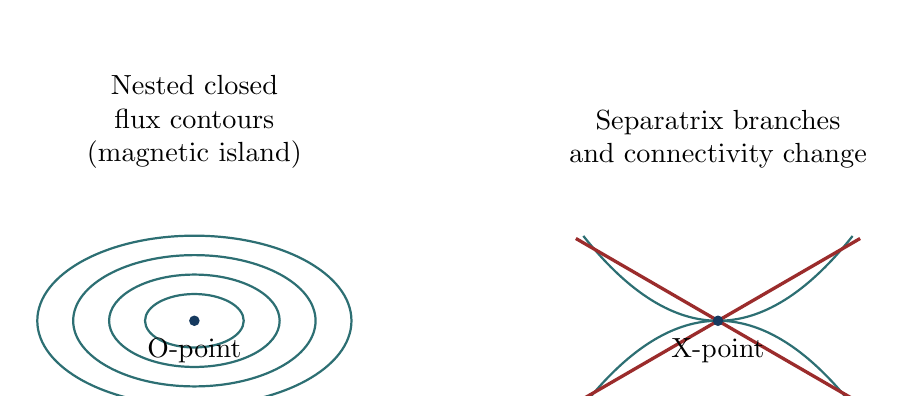
\begin{tikzpicture}[scale=0.95]
  \begin{scope}[xshift=-3.5cm]
    \foreach \r in {0.55,0.95,1.35,1.75} {
      \draw[AccentTeal,thick] (0,0) ellipse ({1.2*\r} and {0.65*\r});
    }
    \fill[TitleBlue] (0,0) circle (2pt);
    \node[below=3pt] at (0,0) {O-point};
    \node[above=7pt,text width=4cm,align=center] at (0,1.65) {Nested closed flux contours\\(magnetic island)};
  \end{scope}
  \begin{scope}[xshift=3.5cm]
    \draw[AccentTeal,thick,domain=-1.8:1.8,samples=80] plot (\x,{0.35*\x*\x});
    \draw[AccentTeal,thick,domain=-1.8:1.8,samples=80] plot (\x,{-0.35*\x*\x});
    \draw[WarningRed,very thick] (-1.9,-1.1)--(1.9,1.1);
    \draw[WarningRed,very thick] (-1.9,1.1)--(1.9,-1.1);
    \fill[TitleBlue] (0,0) circle (2pt);
    \node[below=3pt] at (0,0) {X-point};
    \node[above=7pt,text width=4cm,align=center] at (0,1.65) {Separatrix branches\\and connectivity change};
  \end{scope}
\end{tikzpicture}
\caption{Conceptual contour structures. Actual project contours need not be ellipses or parabolas. An island is a region of closed magnetic-flux contours around an O-point; an X-point lies on the separatrix.}
\label{fig:oxpoints}
\end{figure}

\subsection{Frozen topology in the ideal model}

When $\eta=0$,
\begin{equation}
\frac{D\psi}{Dt}=0.
\end{equation}
Every fluid element preserves its value of $\psi$. Because the flow is smooth and incompressible, it continuously deforms flux contours but cannot cut and reconnect them. Magnetic field lines are said to be \emph{frozen into} the fluid.

Flux freezing is a statement about topology and material transport, not a statement that the magnetic field is spatially or temporally constant. Ideal motion can stretch field lines, rotate them, amplify gradients, and form current sheets while preserving connectivity.

\subsection{How resistivity enables reconnection}

At finite $\eta$,
\begin{equation}
\frac{D\psi}{Dt}=\eta\nabla^2\psi=-\eta J.
\end{equation}
The value of $\psi$ attached to a moving fluid element can change. In a thin current sheet, $|J|=|\nabla^2\psi|$ becomes large enough that $\eta J$ remains dynamically important even if $\eta\ll1$. Flux contours can then change connectivity near an X-point. This process is magnetic reconnection.

From Eq.~\eqref{eq:Ezpsit}, the out-of-plane electric field in the adopted gauge is $E_z=-\psi_t$ in dimensional variables. At a reconnection site, the non-ideal electric field is closely connected to the rate at which flux changes. Exact signs of a reported ``reconnection rate'' depend on which difference of O-point and X-point flux is defined, so Module~2 must record that diagnostic definition explicitly.

\subsection{Current-sheet formation}

The ideal terms can drive initially smooth fields toward smaller spatial scales. Since
\begin{equation}
J=-\nabla^2\psi,
\end{equation}
strong curvature of the flux function produces large current. Diffusion acts increasingly strongly as the length scale shrinks. A useful order-of-magnitude balance across a sheet of thickness $\delta$ is
\begin{equation}
\eta\nabla^2\psi\sim\eta\frac{\psi}{\delta^2}.
\end{equation}
Thus a small global diffusivity does not imply a negligible local resistive term.

\subsection{Magnetic islands and coalescence}

A magnetic island consists of closed flux contours around an O-point, bounded by a separatrix passing through one or more X-points. Parallel out-of-plane current channels can attract through the Lorentz force. Their magnetic islands are advected toward one another, a current sheet forms between them, reconnection changes the connectivity, and the islands merge into a larger structure. This is the \emph{island-coalescence} process selected for Module~2.

The benchmark is valuable because it simultaneously exercises:
\begin{itemize}
  \item nonlinear flux advection $[U,\psi]$;
  \item nonlinear vorticity advection $[U,\omega]$;
  \item Lorentz forcing $[J,\psi]$;
  \item current-sheet formation;
  \item resistive topology change;
  \item viscous damping; and
  \item parameter sensitivity to $\eta$, $\nu$, and perturbation amplitude $A_0$.
\end{itemize}

The exact equilibrium and perturbation formulas, the number and placement of islands, and the operational definition of reconnected flux belong to Module~2. Module~1 establishes only the physics and conventions needed to interpret them.

\subsection{A qualitative Sweet-Parker scale estimate}

In a steady two-dimensional reconnection layer of length $L_s$ and thickness $\delta_s$, incompressible mass conservation suggests
\begin{equation}
V_{\rm in}L_s\sim V_{\rm out}\delta_s,
\end{equation}
where $V_{\rm in}$ and $V_{\rm out}$ are inflow and outflow speeds. Balancing advective and resistive terms in the induction equation suggests
\begin{equation}
V_{\rm in}\frac{B}{\delta_s}
\sim
\eta_{\rm m}\frac{B}{\delta_s^2},
\qquad
V_{\rm in}\sim\frac{\eta_{\rm m}}{\delta_s}.
\end{equation}
If $V_{\rm out}$ is of order the Alfv\'en speed, these estimates give
\begin{equation}
\frac{\delta_s}{L_s}\sim S_s^{-1/2},
\qquad
\frac{V_{\rm in}}{V_A}\sim S_s^{-1/2},
\end{equation}
where $S_s=L_sV_A/\eta_{\rm m}$ is based on sheet length. This is the classical Sweet-Parker scaling. It is an explanatory estimate, not an assumed law for every transient coalescence trajectory. At sufficiently large Lundquist number, secondary islands and unsteady dynamics may invalidate the single steady-sheet picture \cite{Goedbloed2010}.

\section{From equations to physics-informed residuals}
\label{sec:pinnresiduals}

\subsection{What an equation residual means}

A field is an exact solution of a partial differential equation (PDE) if substitution makes the left-minus-right difference zero everywhere in its domain. This difference is the \emph{residual}. For predicted fields $\psi_\theta$ and $U_\theta$, where $\theta$ denotes neural-network parameters, define
\begin{align}
J_\theta&=-\Lap\psi_\theta,\\
\omega_\theta&=\Lap U_\theta.
\end{align}
The frozen \emph{strong-form} residuals, meaning the differential equations evaluated point by point, are
\begin{align}
\boxed{
\Rpsi
=\frac{\partial\psi_\theta}{\partial t}
+\bracket{U_\theta}{\psi_\theta}
-\eta\Lap\psi_\theta,}
\label{eq:Rpsi}\\[0.4em]
\boxed{
\Romega
=\frac{\partial\omega_\theta}{\partial t}
+\bracket{U_\theta}{\omega_\theta}
-\bracket{J_\theta}{\psi_\theta}
-\nu\Lap\omega_\theta.}
\label{eq:Romega}
\end{align}
An exact smooth solution has $\Rpsi=\Romega=0$.

\subsection{Residual losses do not replace data automatically}

Using IC for \emph{initial condition} and BC for \emph{boundary condition}, a typical PINN objective contains
\begin{equation}
\mathcal{L}
=w_{\rm data}\mathcal{L}_{\rm data}
+w_{\rm PDE}\mathcal{L}_{\rm PDE}
+w_{\rm IC}\mathcal{L}_{\rm IC}
+w_{\rm BC}\mathcal{L}_{\rm BC}
+w_{\rm global}\mathcal{L}_{\rm global}.
\end{equation}
Here:
\begin{itemize}
  \item $\mathcal{L}_{\rm data}$ compares predictions with sampled synthetic fields;
  \item $\mathcal{L}_{\rm PDE}$ penalizes $\Rpsi$ and $\Romega$ at collocation points, which are sampled space-time-parameter points where the residual is evaluated;
  \item $\mathcal{L}_{\rm IC}$ enforces the initial condition;
  \item $\mathcal{L}_{\rm BC}$ enforces periodic values and required derivatives;
  \item $\mathcal{L}_{\rm global}$ may penalize violations of energy, means, or other integral identities; and
  \item the nonnegative $w$ values are loss weights.
\end{itemize}
The physics loss narrows the admissible function space, but the PDE alone does not select a unique trajectory without initial conditions, boundary conditions, parameters, and gauge constraints.

\subsection{Derivative order in the direct $(\psi,U)$ formulation}

The direct residual is more demanding than its compact notation suggests. Substituting $J=-\nabla^2\psi$ and $\omega=\nabla^2U$ into Eq.~\eqref{eq:Romega} produces:
\begin{itemize}
  \item the mixed derivative $\partial_t\nabla^2U$;
  \item third spatial derivatives of $\psi$ inside $[J,\psi]$; and
  \item fourth spatial derivatives of $U$ inside $\nabla^2\omega=\nabla^4U$.
\end{itemize}
Automatic differentiation, an algorithm that differentiates the neural computational graph by repeated chain rules, can compute these derivatives. High-order derivatives can nevertheless be noisy to optimize and expensive to evaluate.

An alternative auxiliary-field formulation predicts $(\psi,U,J,\omega)$ and adds definition residuals
\begin{equation}
\mathcal{R}_J=J+\nabla^2\psi,
\qquad
\mathcal{R}_{\omega,\rm def}=\omega-\nabla^2U.
\end{equation}
Then the evolution residuals require at most first derivatives of $J$ and second derivatives of $\omega$. This changes the neural architecture and loss design, not the underlying physics. The version-1 project map remains
\begin{equation}
(x,y,t,\eta,\nu,A_0)\longmapsto(\psi,U)
\end{equation}
unless a later implementation decision is explicitly versioned.

\subsection{Periodic and gauge residuals}

For direct coordinate inputs, periodic losses may include
\begin{align}
\psi(0,y,t)-\psi(L_x,y,t)&=0,\\
U(0,y,t)-U(L_x,y,t)&=0,
\end{align}
and analogous $y$-face equations. Because the PDE contains high derivatives, matching relevant derivatives across the faces is also necessary unless periodicity is built into the network representation, for example through sine-cosine features.

The gauge constraint may be enforced by subtracting the spatial mean of $U$ or by a loss on $\average{U}$. The mean of $\psi$ must remain consistent with the selected case metadata.

\subsection{Global balance as a diagnostic or loss}

For predicted fields, define the energy-balance defect
\begin{equation}
\mathcal{R}_E(t)
=\frac{\dd}{\dd t}(E_B+E_K)
+\eta\int_\Omega J^2\,\dd A
+\nu\int_\Omega\omega^2\,\dd A.
\end{equation}
An exact solution has $\mathcal{R}_E=0$. A global loss can penalize sampled values of $\mathcal{R}_E$, but it cannot replace pointwise PDE residuals: many incorrect fields can share the same total energy history.

\subsection{Parameter conditioning}

The coefficients $\eta$, $\nu$, and $A_0$ are inputs, not trainable physical constants in the initial parameterized surrogate. Whole parameter combinations must be held out for testing. If randomly selected space-time points from every trajectory are placed in both training and test sets, the test does not demonstrate generalization to an unseen physical case.

\begin{warningbox}
A small numerical PDE loss is not, by itself, proof of physical accuracy. Residual sampling may miss localized current sheets; a network may satisfy a modified equation because derivative scaling is wrong; and a low unweighted residual can hide an inaccurate high-order field such as $J$. Validation must include field errors, derived-field errors, global balances, and held-out parameter cases.
\end{warningbox}

\section{Relationship to M3D-C1}
\label{sec:m3dc1relation}

\subsection{What M3D-C1 is}

M3D-C1 is an initial-value, high-order finite-element code for nonlinear extended-MHD calculations in magnetized plasmas. The official overview describes models for density, fluid velocity, total and electron pressures, generalized Ohm's law, magnetic evolution, anisotropic transport, viscous stresses, sources, and optional two-fluid terms. It uses unstructured high-order $C^1$ elements and implicit or semi-implicit time integration to address disparate spatial and temporal scales \cite{M3DC1overview,Jardin2008}.

M3D-C1 also provides reduced representations based on scalar potentials. In cylindrical coordinates $(R,\varphi,Z)$, where $R$ is major-radius coordinate, $\varphi$ is toroidal angle, and $Z$ is vertical coordinate, its magnetic field can be represented schematically using a poloidal-flux variable $\psi$ and a toroidal-field variable. A two-field reduced option retains flux-like and stream-function-like fields called $\psi$ and $U$ \cite{M3DC1overview}.

\subsection{Conceptual connection without false equivalence}

Our Cartesian potentials and the M3D-C1 reduced potentials share a concept: represent divergence-constrained vector fields using scalar functions and evolve a smaller field set. They are not numerically identical variables. M3D-C1 uses toroidal geometry, code-specific normalization, finite-element bases, and model options absent here. A later adapter must establish an explicit mapping from exported M3D-C1 quantities to any learning variables.

\begin{longtable}{p{0.22\textwidth}p{0.32\textwidth}p{0.36\textwidth}}
\toprule
Feature & Version-1 synthetic model & M3D-C1 capability or context \\
\midrule
\endfirsthead
\toprule
Feature & Version-1 synthetic model & M3D-C1 capability or context \\
\midrule
\endhead
Geometry & 2D Cartesian periodic square & Cylindrical/toroidal geometry; axisymmetric and fully 3D modes \\
Primary dynamics & Two scalar fields $\psi,U$ & Single-fluid, two-fluid, and reduced model options with more fields \\
Density & Constant and not evolved & Evolved density in general models \\
Pressure/temperature & Not evolved & Total/electron pressure and thermal transport options \\
Magnetic field & Uniform guide field plus in-plane flux field & General toroidal magnetic representation \\
Flow & In-plane incompressible flow & More general velocity decomposition and compressible dynamics \\
Non-ideal physics & Constant scalar $\eta$ and $\nu$ & Resistivity, stress models, two-fluid terms, transport, sources, and additional closures \\
Boundary & Doubly periodic & Plasma, vacuum, wall, and free-boundary capabilities depending on problem \\
Spatial method & Planned Fourier pseudo-spectral solver & High-order unstructured $C^1$ finite elements \\
Time advance & Selected and verified in Module~2 & Implicit and semi-implicit methods \\
Data status & Independently generated synthetic fields & Genuine code exports require licensed runs or provided data \\
Scientific claim & Reduced-MHD PINN proof of concept & No validated M3D-C1 surrogate claim without genuine data \\
\bottomrule
\end{longtable}

\subsection{What the proof of concept legitimately demonstrates}

If successful, the project can show that a parameterized neural surrogate can learn nonlinear resistive-MHD field evolution while being constrained by a stated PDE, initial conditions, periodic boundaries, and global balances. It can also establish versioned metadata, held-out case splits, diagnostics, and an export schema suitable for later replacement of synthetic trajectories by genuine M3D-C1 results.

It cannot establish that the neural network predicts toroidal extended-MHD behavior, pressure-driven modes, two-fluid dynamics, stellarator geometry, wall interaction, or M3D-C1 numerical errors. Those are separate scientific questions.

\section{Worked analytic examples}
\label{sec:examples}

These examples are intentionally simple. Their purpose is to turn the definitions into calculable objects and to provide future unit or manufactured-solution tests.

\subsection{Example 1: a single magnetic Fourier mode}

Let
\begin{equation}
\psi(x,y)=A\cos(k_xx)\cos(k_yy),
\qquad U=0,
\label{eq:singlepsimode}
\end{equation}
where $A$ is a constant amplitude and $k_x,k_y$ are wavenumbers compatible with the periodic box. Then
\begin{align}
B_x&=\psi_y=-A k_y\cos(k_xx)\sin(k_yy),\\
B_y&=-\psi_x=+A k_x\sin(k_xx)\cos(k_yy),\\
J&=-\nabla^2\psi=(k_x^2+k_y^2)\psi.
\end{align}
Because $J$ is proportional to $\psi$,
\begin{equation}
[J,\psi]=0.
\end{equation}
There is no vorticity generation. The flux equation reduces to diffusion:
\begin{equation}
\psi_t=-\eta(k_x^2+k_y^2)\psi.
\end{equation}
The exact solution is
\begin{equation}
\boxed{
\psi(x,y,t)=A\exp[-\eta(k_x^2+k_y^2)t]
\cos(k_xx)\cos(k_yy),
\qquad U=0.}
\label{eq:psidecaysolution}
\end{equation}
This solution checks spectral derivatives, current sign, resistive decay rate, and time integration.

\subsection{Example 2: a single viscously decaying flow mode}

Let
\begin{equation}
U(x,y,t)=C(t)\cos(k_xx)\cos(k_yy),
\qquad\psi=0.
\end{equation}
Then
\begin{align}
v_x&=C(t)k_y\cos(k_xx)\sin(k_yy),\\
v_y&=-C(t)k_x\sin(k_xx)\cos(k_yy),\\
\omega&=-(k_x^2+k_y^2)U.
\end{align}
Because $\omega$ is proportional to $U$, $[U,\omega]=0$. The vorticity equation becomes
\begin{equation}
\omega_t=\nu\nabla^2\omega,
\end{equation}
which implies
\begin{equation}
\boxed{C(t)=C(0)\exp[-\nu(k_x^2+k_y^2)t].}
\end{equation}
This checks stream-function signs, vorticity, Poisson inversion, and viscous decay.

\subsection{Example 3: the bracket as advection}

Choose
\begin{equation}
U=\sin x\sin y,
\qquad f=\cos x.
\end{equation}
Then
\begin{align}
\vect{v}&=(-U_y,U_x)=(-\sin x\cos y,\cos x\sin y),\\
\vect{v}\cdot\nabla f
&=(-\sin x\cos y)(-\sin x)
+(\cos x\sin y)(0)\\
&=\sin^2x\cos y.
\end{align}
Directly from the bracket,
\begin{align}
[U,f]&=U_xf_y-U_yf_x\\
&=(\cos x\sin y)(0)-(\sin x\cos y)(-\sin x)\\
&=\sin^2x\cos y.
\end{align}
The results match, verifying Eq.~\eqref{eq:vadvectionbracket}.

\subsection{Example 4: an ideal static equilibrium family}

Let $U=0$ and suppose
\begin{equation}
J=F(\psi)
\end{equation}
for any differentiable single-valued function $F$. Then
\begin{equation}
[J,\psi]=F'(\psi)[\psi,\psi]=0.
\end{equation}
With $\eta=\nu=0$, both evolution equations are satisfied. This is the curl-level equilibrium condition. The pressure field removed by the curl may still be needed to balance the gradient part of the Lorentz force in the original momentum equation.

\subsection{Example 5: energy decay of the magnetic mode}

For the exact solution in Eq.~\eqref{eq:psidecaysolution}, magnetic energy is proportional to the squared amplitude:
\begin{equation}
E_B(t)=E_B(0)\exp[-2\eta(k_x^2+k_y^2)t].
\end{equation}
The energy law predicts
\begin{equation}
\frac{\dd E_B}{\dd t}=-\eta\int J^2\,\dd A.
\end{equation}
Since $J=k^2\psi$ and $\int|\nabla\psi|^2\dd A=k^2\int\psi^2\dd A$, the right-hand side equals $-2\eta k^2E_B$, exactly matching the time derivative. Here $k^2=k_x^2+k_y^2$.

\section{Verification identities and mandatory convention tests}
\label{sec:verification}

The following checks should be implemented before island-coalescence data is accepted as a learning target.

\subsection{Differential identity tests}

For known Fourier modes, verify:
\begin{enumerate}[label=\arabic*.]
  \item first and second spatial derivatives at their expected convergence rate;
  \item $\nabla\cdot\vect{B}_\perp=0$ and $\nabla\cdot\vect{v}_\perp=0$ near numerical precision;
  \item $J=-\nabla^2\psi$ and $\omega=+\nabla^2U$;
  \item bracket antisymmetry, $[f,g]+[g,f]=0$;
  \item self-bracket, $[f,f]=0$;
  \item the cyclic integral identity in Eq.~\eqref{eq:bracketcyclic}; and
  \item periodic matching of fields and derivatives.
\end{enumerate}

\subsection{Analytic evolution tests}

Use Eqs.~\eqref{eq:psidecaysolution} and its viscous counterpart to verify:
\begin{itemize}
  \item exponential amplitude decay rate;
  \item correct independence of magnetic decay from $\nu$ in the no-flow case;
  \item correct independence of flow decay from $\eta$ in the no-field case;
  \item convergence under grid refinement;
  \item convergence under time-step refinement; and
  \item preservation of all inactive fields at roundoff or truncation level.
\end{itemize}

\subsection{Integral-balance tests}

Track
\begin{align}
E_B(t),\quad E_K(t),\quad
\int J^2\dd A,\quad\int\omega^2\dd A,
\quad\average{\psi},\quad\average{U},
\quad\average{J},\quad\average{\omega}.
\end{align}
The discrete energy defect over a time interval $[t_a,t_b]$ can be evaluated as
\begin{equation}
\epsilon_E
=E(t_b)-E(t_a)
+\int_{t_a}^{t_b}\left[
\eta\int_\Omega J^2\dd A
+\nu\int_\Omega\omega^2\dd A
\right]\dd t.
\end{equation}
For a convergent consistent solver, $\epsilon_E$ should approach zero as spatial and temporal resolution increase.

\subsection{Why visual plausibility is insufficient}

Contour plots can look physically reasonable even when a current sign is reversed, a derivative is aliased, or energy grows spuriously. Verification must use exact identities and convergence, not only images. Conversely, a thin current sheet that appears noisy may be under-resolved rather than physically turbulent. Resolution studies distinguish these possibilities.

\begin{longtable}{p{0.27\textwidth}p{0.25\textwidth}p{0.38\textwidth}}
\toprule
Check & Expected result & Likely failure indicated \\
\midrule
\endfirsthead
\toprule
Check & Expected result & Likely failure indicated \\
\midrule
\endhead
$\nabla\cdot\vect{B}$ & Near numerical precision & Flux-to-field derivative inconsistency \\
$\nabla\cdot\vect{v}$ & Near numerical precision & Stream-to-velocity derivative inconsistency \\
$[f,g]+[g,f]$ & Near zero & Bracket implementation or axis-order error \\
$\average{U}$ & Exactly or nearly zero & Uncontrolled Poisson zero mode \\
$\average{\psi}$ & Constant & Mean-mode drift or inconsistent gauge handling \\
$E(t)$ for $\eta,\nu>0$ & Nonincreasing & Sign error, forcing, or numerical instability \\
Analytic Fourier decay & Correct exponent & Diffusion sign, wavenumber, or time-scale error \\
Refinement study & Error decreases & Under-resolution or inconsistent discretization \\
\bottomrule
\end{longtable}

\section{Common misconceptions and sign traps}
\label{sec:misconceptions}

\subsection{``$\psi$ is the magnetic field''}

No. $\psi$ is a scalar potential. The in-plane magnetic field is made from its first derivatives. A spatially constant $\psi$ produces zero in-plane magnetic field.

\subsection{``$U$ is a velocity component''}

No. $U$ is a stream function with velocity obtained from first derivatives. Adding a spatial constant to $U$ changes no physical velocity.

\subsection{``$J$ is the current density in amperes per square meter''}

Not in the nondimensional project. Physical current density is
\begin{equation}
j_{z,\rm d}=\frac{B_0}{\mu_0L_0}J.
\end{equation}
The project $J$ is dimensionless.

\subsection{``Resistivity and magnetic diffusivity have the same units''}

No. Electrical resistivity $\rho_\Omega$ has units $\unit{\Omega\,m}$. Magnetic diffusivity $\eta_{\rm m}=\rho_\Omega/\mu_0$ has units $\unit{m^2\,s^{-1}}$. Project $\eta$ is dimensionless.

\subsection{``A small $\eta$ can be ignored everywhere''}

No. The relevant term is $\eta\nabla^2\psi=-\eta J$. Current density can become large in a thin sheet, making the product finite and controlling topology change.

\subsection{``Incompressible means motionless or uniform''}

No. It means $\nabla\cdot\vect{v}=0$. Incompressible flows can be nonlinear, vortical, and turbulent.

\subsection{``Two-dimensional means every vector has two components''}

No. Two-dimensional means fields are independent of one coordinate. Current and vorticity point in the ignorable $z$ direction even though magnetic and velocity perturbations lie in the plane.

\subsection{``Pressure was set to zero''}

No. Its gradient was eliminated by taking the curl under constant density. Pressure still enforces incompressibility in the parent momentum equation.

\subsection{``Reduced MHD and full M3D-C1 are the same equations''}

No. M3D-C1 supports far richer geometry, field content, transport, and closures. Shared variable names do not imply numerical identity.

\subsection{``A PINN residual is just another regression error''}

Not exactly. It measures violation of a differential equation. Its magnitude depends on derivative scales, normalization, and sampling. A residual can be small for the wrong equation if chain-rule factors or signs are incorrect.

\subsection{``Numerical diffusion and physical diffusion are interchangeable''}

No. The parameters $\eta$ and $\nu$ represent explicit model transport. Discretization also introduces truncation error and may introduce numerical dissipation. The latter must be shown to decrease with refinement and should not silently replace the specified physics.

\section{Module-1 computational contract}
\label{sec:contract}

The following statements constitute the handoff from physics notes to later implementation.

\subsection{State and parameter contract}

\begin{align}
\text{Inputs: }&(x,y,t,\eta,\nu,A_0),\\
\text{Primary outputs: }&(\psi,U),\\
\text{Derived outputs: }&J=-\nabla^2\psi,\quad\omega=\nabla^2U.
\end{align}
All are dimensionless in version~1. Dimensional reference scales must remain in metadata even when assigned numerical value one.

\subsection{Equation contract}

\begin{align}
\psi_t+[U,\psi]-\eta\nabla^2\psi&=0,\\
\omega_t+[U,\omega]-[J,\psi]-\nu\nabla^2\omega&=0,\\
[f,g]&=f_xg_y-f_yg_x.
\end{align}

\subsection{Boundary and gauge contract}

\begin{itemize}
  \item $\psi$, $U$, and required derivatives are periodic in $x$ and $y$.
  \item $\average{U}=0$ at every stored time.
  \item $\average{\psi}$ is recorded and remains constant within a case.
  \item The $\vect{k}=0$ mode is handled explicitly in every Poisson inversion.
\end{itemize}

\subsection{Diagnostic contract}

At minimum, store or compute:
\begin{itemize}
  \item magnetic energy $E_B$;
  \item kinetic energy $E_K$;
  \item total energy $E_B+E_K$;
  \item peak current $\max_{\Omega}|J|$;
  \item Ohmic dissipation rate $\eta\int J^2\dd A$;
  \item viscous dissipation rate $\nu\int\omega^2\dd A$;
  \item mean and gauge checks;
  \item reconnected flux using a versioned O-point/X-point definition; and
  \item PDE residuals for learned fields.
\end{itemize}

\subsection{Required provenance}

Each generated case must preserve the domain, grid, time array, coefficients, initial-condition parameters, normalization scales, sign-convention version, solver version, boundary conditions, field names, and diagnostic definitions. A contour image is not a scientific dataset.

\section{Summary and bridge to Module 2}
\label{sec:summary}

The project begins from a conducting one-fluid description and then imposes constant density, incompressibility, two-dimensional Cartesian geometry, a uniform guide field, scalar resistivity and viscosity, and periodic boundaries. Divergence-free in-plane fields are represented by a flux function and stream function:
\begin{equation}
\vect{B}_\perp=(\psi_y,-\psi_x),
\qquad
\vect{v}_\perp=(-U_y,U_x).
\end{equation}
These choices fix
\begin{equation}
J=-\nabla^2\psi,
\qquad
\omega=+\nabla^2U.
\end{equation}
Two-dimensional advection is represented by
\begin{equation}
[f,g]=f_xg_y-f_yg_x.
\end{equation}
The final dimensionless system is
\begin{align}
\psi_t+[U,\psi]&=\eta\nabla^2\psi,\\
\omega_t+[U,\omega]&=[J,\psi]+\nu\nabla^2\omega.
\end{align}
The ideal nonlinear terms exchange magnetic and kinetic energy but do not change their sum. On the periodic domain,
\begin{equation}
\frac{\dd}{\dd t}(E_B+E_K)
=-\eta\int J^2\dd A-\nu\int\omega^2\dd A.
\end{equation}
Finite resistivity breaks frozen-in flux in regions of high current, enabling reconnection and magnetic-island coalescence.

Module~2 must now supply what Module~1 intentionally does not: a precise island-coalescence equilibrium and perturbation; pseudo-spectral spatial discretization; de-aliasing (removal of spurious unresolved Fourier-mode interactions); time integration; case parameter ranges; convergence criteria; and a versioned definition of reconnected flux. No synthetic trajectory should be used for neural training until the analytic decay tests, sign audits, periodic checks, convergence studies, and energy balance described here have passed.

\clearpage
\appendix

\section{Component-by-component sign audit}
\label{app:signaudit}

This appendix repeats the shortest possible audit in one place.

\subsection{Magnetic field and current}

\begin{align}
\vect{B}_\perp
&=\nabla\psi\times\widehat{\vect{z}}\\
&=(\psi_x\widehat{\vect{x}}+\psi_y\widehat{\vect{y}})
\times\widehat{\vect{z}}\\
&=\psi_y\widehat{\vect{x}}-\psi_x\widehat{\vect{y}},\\
(\nabla\times\vect{B})_z
&=\partial_x(-\psi_x)-\partial_y(\psi_y)\\
&=-\nabla^2\psi.
\end{align}
Therefore $J=-\nabla^2\psi$.

\subsection{Velocity and vorticity}

\begin{align}
\vect{v}_\perp
&=\widehat{\vect{z}}\times\nabla U\\
&=-U_y\widehat{\vect{x}}+U_x\widehat{\vect{y}},\\
(\nabla\times\vect{v})_z
&=\partial_x(U_x)-\partial_y(-U_y)\\
&=+\nabla^2U.
\end{align}
Therefore $\omega=+\nabla^2U$.

\subsection{Advection}

\begin{equation}
\vect{v}\cdot\nabla f
=(-U_y)f_x+(U_x)f_y
=[U,f].
\end{equation}

\subsection{Flux equation}

\begin{align}
(\vect{v}\times\vect{B})_z
&=v_xB_y-v_yB_x\\
&=(-U_y)(-\psi_x)-(U_x)(\psi_y)\\
&=-[U,\psi],\\
E_z+(\vect{v}\times\vect{B})_z
&=\rho_\Omega j_z,\\
-\psi_t-[U,\psi]&=-\eta_{\rm m}\nabla^2\psi,\\
\psi_t+[U,\psi]&=+\eta_{\rm m}\nabla^2\psi.
\end{align}

\subsection{Lorentz bracket}

\begin{align}
\vect{j}\times\vect{B}
&=j_z\widehat{\vect{z}}\times(\psi_y,-\psi_x,0)\\
&=j_z(\psi_x,\psi_y,0)\\
&=j_z\nabla\psi,\\
[\nabla\times(j_z\nabla\psi)]_z
&=(j_z)_x\psi_y-(j_z)_y\psi_x\\
&=[j_z,\psi].
\end{align}
Alfv\'en normalization maps the physical current density to $J$ and produces $+[J,\psi]$ in the vorticity equation.

\section{Vector and integral identities used in the energy proof}
\label{app:identities}

For smooth periodic scalar fields $f$ and $g$,
\begin{align}
\int_\Omega f\nabla^2g\,\dd A
&=-\int_\Omega\nabla f\cdot\nabla g\,\dd A\\
&=\int_\Omega g\nabla^2f\,\dd A.
\end{align}
Thus the periodic Laplacian is self-adjoint.

For smooth periodic $f,g,h$,
\begin{align}
\int_\Omega f[g,h]\,\dd A
&=\int_\Omega f(g_xh_y-g_yh_x)\,\dd A\\
&=-\int_\Omega g\left(f_xh_y-f_yh_x\right)\,\dd A\\
&=\int_\Omega g[h,f]\,\dd A.
\end{align}
The omitted boundary terms vanish by periodicity. Repeating the permutation gives the full cyclic identity.

\section{Symbol table}
\label{app:symbols}

\small
\begin{longtable}{p{0.16\textwidth}p{0.50\textwidth}p{0.23\textwidth}}
\toprule
Symbol & Meaning & Units or status \\
\midrule
\endfirsthead
\toprule
Symbol & Meaning & Units or status \\
\midrule
\endhead
$x,y,z$ & Cartesian coordinates after physical nondimensionalization & dimensionless \\
$x_{\rm d},y_{\rm d},z_{\rm d}$ & Dimensional Cartesian coordinates & $\unit{m}$ \\
$t,t_{\rm d}$ & Dimensionless and dimensional time & $1$ and $\unit{s}$ \\
$\Omega$ & Periodic two-dimensional domain & dimensionless area \\
$L_x,L_y$ & Dimensionless domain lengths & dimensionless \\
$L_0$ & Dimensional reference length & $\unit{m}$ \\
$\widehat{\vect{x}},\widehat{\vect{y}},\widehat{\vect{z}}$ & Cartesian unit vectors & dimensionless \\
$\nabla,\nabla^2$ & Gradient and Laplacian in dimensionless coordinates & dimensionless operators \\
$\partial_t$ & Partial derivative at fixed spatial position & inverse dimensionless time \\
$D/Dt$ & Material derivative following the fluid & inverse time \\
$[f,g]$ & Poisson bracket $f_xg_y-f_yg_x$ & depends on $f,g$ \\
$\rho_{\rm d}$ & Mass density & $\unit{kg\,m^{-3}}$ \\
$\rho_0$ & Constant reference mass density & $\unit{kg\,m^{-3}}$ \\
$n_i,n_e$ & Ion and electron number density & $\unit{m^{-3}}$ \\
$m_i,m_e$ & Ion and electron mass & $\unit{kg}$ \\
$e$ & Positive elementary-charge magnitude & $\unit{C}$ \\
$p_{\rm d}$ & Isotropic fluid pressure & $\unit{Pa}$ \\
$\gamma$ & Ratio of specific heats & dimensionless \\
$\vect{E}_{\rm d}$ & Electric field & $\unit{V\,m^{-1}}$ \\
$\vect{B}_{\rm d}$ & Magnetic field & $\unit{T}$ \\
$B_g$ & Constant out-of-plane guide field & $\unit{T}$ \\
$B_0$ & Reference in-plane magnetic-field scale & $\unit{T}$ \\
$\vect{j}_{\rm d}$ & Electric current density & $\unit{A\,m^{-2}}$ \\
$j_{z,\rm d}$ & Out-of-plane current-density component & $\unit{A\,m^{-2}}$ \\
$\mu_0$ & Permeability of free space & $\unit{N\,A^{-2}}$ \\
$\rho_\Omega$ & Electrical resistivity & $\unit{\Omega\,m}$ \\
$\eta_{\rm m}$ & Magnetic diffusivity $\rho_\Omega/\mu_0$ & $\unit{m^2\,s^{-1}}$ \\
$\eta$ & Project magnetic diffusivity $\eta_{\rm m}/(L_0V_A)$ & dimensionless \\
$\nu_{\rm d}$ & Dimensional kinematic viscosity & $\unit{m^2\,s^{-1}}$ \\
$\nu$ & Project kinematic viscosity $\nu_{\rm d}/(L_0V_A)$ & dimensionless \\
$V_A$ & Alfv\'en speed $B_0/\sqrt{\mu_0\rho_0}$ & $\unit{m\,s^{-1}}$ \\
$t_A$ & Alfv\'en time $L_0/V_A$ & $\unit{s}$ \\
$S$ & Lundquist number $L_0V_A/\eta_{\rm m}$ & dimensionless \\
$\mathrm{Re}$ & Reynolds number $L_0V_A/\nu_{\rm d}$ & dimensionless \\
$\mathrm{Rm}$ & Magnetic Reynolds number $L_0V_0/\eta_{\rm m}$ & dimensionless \\
$\mathrm{Pm}$ & Magnetic Prandtl number $\nu_{\rm d}/\eta_{\rm m}$ & dimensionless \\
$\psi_{\rm d}$ & Dimensional magnetic-flux function & $\unit{T\,m}$ \\
$\psi$ & Dimensionless magnetic-flux function & dimensionless \\
$U_{\rm d}$ & Dimensional flow stream function & $\unit{m^2\,s^{-1}}$ \\
$U$ & Dimensionless flow stream function & dimensionless \\
$J$ & Dimensionless current variable $-\nabla^2\psi$ & dimensionless \\
$\omega$ & Dimensionless out-of-plane vorticity $\nabla^2U$ & dimensionless \\
$E_B,E_K$ & Dimensionless magnetic and kinetic energy integrals & dimensionless \\
$H_C$ & Dimensionless cross helicity & dimensionless \\
$A_0$ & Initial perturbation amplitude parameter & dimensionless \\
$\boldsymbol{\mu}$ & Case parameter vector $(\eta,\nu,A_0)$ & dimensionless \\
$\theta$ & Neural-network trainable parameter vector & numerical parameters \\
$\Rpsi,\Romega$ & Flux and vorticity PDE residuals & dimensionless residuals \\
$\average{f}$ & Spatial mean of $f$ over $\Omega$ & same units as $f$ \\
\bottomrule
\end{longtable}
\normalsize

\section{Acronym and terminology table}
\label{app:acronyms}

\begin{longtable}{p{0.18\textwidth}p{0.72\textwidth}}
\toprule
Term & Meaning \\
\midrule
\endfirsthead
\toprule
Term & Meaning \\
\midrule
\endhead
1D, 2D, 3D & One-, two-, and three-dimensional \\
BC & Boundary condition \\
$C^1$ & Continuity class in which a represented field and its first derivatives are continuous \\
FFT & Fast Fourier transform \\
IC & Initial condition \\
M3D-C1 & Code name for a high-order extended-MHD simulation framework; C1 refers to $C^1$ elements \\
MHD & Magnetohydrodynamics \\
O-point & Magnetic critical point at the center of nested closed flux contours \\
PDE & Partial differential equation \\
PINN & Physics-informed neural network \\
RMHD & Reduced magnetohydrodynamics; the exact reduction must always be stated \\
SI & International System of Units \\
X-point & Saddle-type magnetic critical point on a separatrix \\
Alfv\'en speed & Characteristic MHD wave speed $B/\sqrt{\mu_0\rho}$ \\
Advection & Transport by bulk fluid motion \\
Diffusion & Smoothing driven by spatial curvature and a diffusivity \\
Flux freezing & Ideal-MHD preservation of magnetic flux attached to moving fluid elements \\
Guide field & Strong magnetic-field component in the ignorable direction \\
Magnetic island & Region of closed flux contours surrounding an O-point \\
Magnetic reconnection & Non-ideal change of magnetic-field-line connectivity \\
Material derivative & Time rate of change following a moving fluid element \\
Separatrix & Flux contour separating topologically distinct field-line regions \\
Stream function & Scalar potential whose rotated gradient produces incompressible 2D velocity \\
Vorticity & Curl of velocity; local rotational content of the flow \\
\bottomrule
\end{longtable}

\section{Concept questions and answer sketches}
\label{app:questions}

\subsection*{Questions}

\begin{enumerate}[label=\textbf{Q\arabic*.}]
  \item Why is MHD a fluid theory even though its derivation begins from kinetic equations?
  \item What is the physical difference between bulk velocity and electric current density?
  \item Why does writing $\vect{B}_\perp=\nabla\psi\times\widehat{\vect{z}}$ guarantee $\nabla\cdot\vect{B}=0$?
  \item With the frozen convention, why does current have a minus sign but vorticity a plus sign?
  \item Show directly that $[U,f]=\vect{v}\cdot\nabla f$.
  \item What happens to $\psi$ following a fluid element when $\eta=0$?
  \item Why can a small resistivity control the evolution inside a current sheet?
  \item Why does pressure disappear from the vorticity equation?
  \item What does the term $[J,\psi]$ represent physically?
  \item Why is the mean of $U$ a gauge choice?
  \item Why must the zero Fourier mode be treated separately when solving $\nabla^2U=\omega$?
  \item Which nonlinear term transfers energy between magnetic and kinetic reservoirs?
  \item Why can total energy only decrease for $\eta,\nu>0$ in the unforced periodic model?
  \item Why is neural min-max scaling not the same as physical nondimensionalization?
  \item Why would a random point split across every trajectory overstate surrogate generalization?
  \item In what precise sense is this project connected to M3D-C1, and in what sense is it not?
\end{enumerate}

\subsection*{Answer sketches}

\begin{enumerate}[label=\textbf{A\arabic*.}]
  \item MHD evolves a finite set of spatial moments such as density, bulk velocity, pressure, and magnetic field, rather than the full velocity-space distribution functions.
  \item Bulk velocity is mass-weighted common motion. Current density is charge-weighted relative motion of positive and negative species.
  \item It is a curl: $\vect{B}_\perp=\nabla\times(\psi\widehat{\vect{z}})$, and the divergence of any smooth curl is zero.
  \item The magnetic and velocity potentials use opposite cross-product order. Taking their $z$ curls gives $J=-\nabla^2\psi$ and $\omega=+\nabla^2U$.
  \item Substitute $\vect{v}=(-U_y,U_x)$: $\vect{v}\cdot\nabla f=-U_yf_x+U_xf_y=[U,f]$.
  \item Its material derivative is zero; the fluid element retains its flux label, expressing frozen-in topology.
  \item The resistive term is $-\eta J$. A current sheet has very large $J$ because $\psi$ varies over a small thickness.
  \item Under constant density, pressure contributes a pure gradient to acceleration, and curl of a gradient is zero.
  \item It is the out-of-plane curl of the Lorentz force per unit mass and drives vorticity and magnetic-kinetic energy exchange.
  \item Only spatial derivatives of $U$ affect velocity and vorticity. Adding a spatial constant changes neither.
  \item The Laplacian eigenvalue is $-|\vect{k}|^2$, which is zero at $\vect{k}=0$; division is undefined. The gauge sets the mean of $U$.
  \item The domain integral $\int U[J,\psi]\dd A$ appears with opposite signs in magnetic and kinetic energy budgets.
  \item Periodic boundaries remove surface fluxes, the brackets only redistribute, and the remaining sinks are nonnegative $\eta\int J^2$ and $\nu\int\omega^2$.
  \item Physical nondimensionalization defines the PDE coefficients. Neural scaling is an additional coordinate transformation whose chain-rule factors must be included in derivatives.
  \item The model can interpolate within portions of every already-seen trajectory. Holding out whole parameter combinations tests a genuinely unseen physical case.
  \item It demonstrates a two-field reduced-MHD surrogate workflow and data contract conceptually relevant to reduced MHD. It neither runs nor validates the full toroidal extended-MHD code.
\end{enumerate}

\clearpage
\begin{thebibliography}{99}

\bibitem{Goedbloed2004}
J. P. Goedbloed and S. Poedts,
\emph{Principles of Magnetohydrodynamics: With Applications to Laboratory and Astrophysical Plasmas},
Cambridge University Press (2004).
Relevant background: Sections 2.4, 3.4, and 4.1--4.4.

\bibitem{Goedbloed2010}
J. P. Goedbloed, R. Keppens, and S. Poedts,
\emph{Advanced Magnetohydrodynamics: With Applications to Laboratory and Astrophysical Plasmas},
Cambridge University Press (2010).
Relevant background: Sections 14.2 and 14.4, and the reduced-MHD discussion in Section 17.3.

\bibitem{M3DC1overview}
Princeton Plasma Physics Laboratory,
``M3D-C1 Overview,''
\url{https://m3dc1.pppl.gov/m3dc1_overview.html},
accessed 4 August 2026.

\bibitem{Jardin2008}
S. C. Jardin, N. Ferraro, X. Luo, J. Chen, J. Breslau, K. E. Jansen, and M. S. Shephard,
``The M3D-C1 approach to simulating 3D 2-fluid magnetohydrodynamics in magnetic fusion experiments,''
\emph{Journal of Physics: Conference Series} \textbf{125}, 012044 (2008),
\url{https://doi.org/10.1088/1742-6596/125/1/012044}.

\bibitem{Strauss1976}
H. R. Strauss,
``Nonlinear, three-dimensional magnetohydrodynamics of noncircular tokamaks,''
\emph{Physics of Fluids} \textbf{19}, 134--140 (1976),
\url{https://doi.org/10.1063/1.861310}.

\bibitem{Biskamp2000}
D. Biskamp,
\emph{Magnetic Reconnection in Plasmas},
Cambridge University Press (2000).

\end{thebibliography}

\end{document}
